%\documentclass[twocolappendix, trackchanges]{aastex7}
\documentclass[twocolumn, linenumbers, twocolappendix,trackchanges]{aastex7}

% line numbers must be on for submission

% Package imports go here.
\usepackage{glossaries}  % Overriding \label
% not allowed ! \usepackage{glossary-mcols}
\usepackage{amsmath}
\usepackage{textcomp}
\usepackage{gensymb}
\usepackage{graphicx}
\usepackage{mathtools, nccmath}
\usepackage{hyperref}
\usepackage[htt]{hyphenat} % Hyphenate texttt blocks
\usepackage{xspace} % grids of plots
\usepackage{subcaption}
\captionsetup{compatibility=false}
\usepackage{booktabs} % For midrule

% Todo notes
\usepackage[colorinlistoftodos]{todonotes}
\let\Oldtodo\todo
\renewcommand{\todo}[1]{\Oldtodo[inline]{#1}}
\newcommand{\eric}[2][]{\Oldtodo[inline,color=blue, #1]{Eric: #2}}
\newcommand{\bri}[2][]{\Oldtodo[inline,color=purple, #1]{Bri: #2}}
\newcommand{\eli}[2][]{\Oldtodo[inline,color=red, #1]{Eli: #2}}
\newcommand{\james}[2][]{\Oldtodo[inline,color=cyan, #1]{James: #2}}
\newcommand{\leanne}[2][]{\Oldtodo[inline,color=teal, #1]{Leanne: #2}}
\newcommand{\gregory}[2][]{\Oldtodo[inline,color=yellow, #1]{Gregory: #2}}
\newcommand{\jake}[2][]{\Oldtodo[inline,color=orange, #1]{Jake: #2}}
\newcommand{\yusra}[2][]{\Oldtodo[inline,color=green, #1]{Yusra: #2}}

\newcommand{\TODO}[1]{\textcolor{red}{\textbf{TODO:} #1}}

% All figures here
\graphicspath{{./}{figures/}}

% Local commands go here.
\newcommand{\docRef}{RTN-095}
\newcommand{\docUpstreamLocation}{\url{https://github.com/lsst/rtn-095}}
%\providecommand{\secref}[1]{\hyperref[#1]{\autoref{#1}}}
\providecommand{\secref}[1]{\hyperref[#1]{\S\ref{#1}}}
\providecommand{\appref}[1]{\hyperref[#1]{Appendix \ref{#1}}}
\providecommand{\tabref}[1]{\hyperref[#1]{\autoref{#1}}}
\providecommand{\figref}[1]{\hyperref[#1]{\autoref{#1}}}
\providecommand{\eqnref}[1]{\hyperref[#1]{Eq.~\ref{#1}}}
\providecommand{\recref}[1]{\hyperref[#1]{REC-\ref{#1}}}

\newcommand{\degsq}{$\rm deg^{2}$}

% DO NOT EDIT - generated by /Users/leanne/Rubin/repos/lsst-texmf/texmf/../bin/generateAcronyms.py from https://lsst-texmf.lsst.io/.
\newacronym{2D} {2D} {Two-dimensional}
\newacronym{ADC} {ADC} {Analogue-to-Digital Converter}
\newacronym{ADQL} {ADQL} {Astronomical Data Query Language (IVOA standard)}
\newacronym{ADU} {ADU} {Analogue-to-Digital Unit}
\newacronym{AOS} {AOS} {Active Optics System}
\newacronym{API} {API} {Application Programming Interface}
\newacronym{ASPIC} {ASPIC} {Analog Signal Processing Integrated Circuit}
\newacronym{AST} {AST} {\gls{NSF} Division of Astronomical Sciences}
\newacronym{ATLAS} {ATLAS} {Asteroid Terrestrial-impact Last Alert System}
\newacronym{AURA} {AURA} {Association of Universities for Research in Astronomy}
\newacronym{Adam} {Adam} {Adaptive Moment Estimation}
\newglossaryentry{Alert} {name={Alert}, description={A packet of information for each source detected with signal-to-noise ratio > 5 in a difference image by Alert Production, containing measurement and characterization parameters based on the past 12 months of LSST observations plus small cutouts of the single-visit, template, and difference images, distributed via the internet}}
\newglossaryentry{Alert Production} {name={Alert Production}, description={Executing on the Prompt Processing system, the Alert Production payload processes and calibrates incoming images, performs Difference Image Analysis to identify DIASources and DIAObjects, and then packages the resulting alerts for distribution.}}
\newglossaryentry{Alternate Standard Visit} {name={Alternate Standard Visit}, description={A single observation of an LSST field comprised of one 30 second exposure}}
\newglossaryentry{Archive} {name={Archive}, description={The repository for documents required by the NSF to be kept. These include documents related to design and development, construction, integration, test, and operations of the LSST observatory system. The archive is maintained using the enterprise content management system DocuShare, which is accessible through a link on the project website www.project.lsst.org}}
\newglossaryentry{Archive Center} {name={Archive Center}, description={Part of the LSST Data Management System, the LSST archive center is a data center at NCSA that hosts the LSST Archive, which includes released science data and metadata, observatory and engineering data, and supporting software such as the LSST Software Stack}}
\newglossaryentry{Association Pipeline} {name={Association Pipeline}, description={An application that matches detected Sources or DIASources or generated Objects to an existing catalog of Objects, producing a (possibly many-to-many) set of associations and a list of unassociated inputs. Association Pipelines are used in Alert Production after DIASource generation and in the final stages of Data Release processing to ensure continuity of Object identifiers}}
\newglossaryentry{Association of Universities for Research in Astronomy} {name={Association of Universities for Research in Astronomy}, description={ consortium of US institutions and international affiliates that operates world-class astronomical observatories, AURA is the legal entity responsible for managing what it calls independent operating Centers, including LSST, under respective cooperative agreements with the National Science Foundation. AURA assumes fiducial responsibility for the funds provided through those cooperative agreements. AURA also is the legal owner of the AURA Observatory properties in Chile}}
\newacronym{BCE} {BCE} {Before Common Era}
\newglossaryentry{Butler} {name={Butler}, description={A middleware component for persisting and retrieving image datasets (raw or processed), calibration reference data, and catalogs}}
\newacronym{CADC} {CADC} {Canadian Astronomy Data Centre}
\newacronym{CCD} {CCD} {Charge-Coupled Device}
\newacronym{CNRS} {CNRS} {Centre national de la recherche scientifique}
\newacronym{CPU} {CPU} {Central Processing Unit}
\newacronym{CTI} {CTI} {Charge Transfer Inefficiency}
\newacronym{CVMFS} {CVMFS} {CernVM File System}
\newglossaryentry{Camera} {name={Camera}, description={The LSST subsystem responsible for the 3.2-gigapixel LSST camera, which will take more than 800 panoramic images of the sky every night. SLAC leads a consortium of Department of Energy laboratories to design and build the camera sensors, optics, electronics, cryostat, filters and filter exchange mechanism, and camera control system}}
\newglossaryentry{Center} {name={Center}, description={An entity managed by AURA that is responsible for execution of a federally funded project}}
\newglossaryentry{Charge-Coupled Device} {name={Charge-Coupled Device}, description={a particular kind of solid-state sensor for detecting optical-band photons. It is composed of a 2-D array of pixels, and one or more read-out amplifiers}}
\newglossaryentry{Coadd Image} {name={Coadd Image}, description={An image that is the combination of multiple input images. The inputs are aligned to a common projection and pixel grid, corrected to the same photometric scale and zero-point, with bad pixels and artifacts rejected. (Image PSFs may also be matched prior to co-addition.) Coadd Images have had non-astrophysical background removed}}
\newglossaryentry{ComCam} {name={ComCam}, description={The commissioning camera is a single-raft, 9-CCD camera that will be installed in LSST during commissioning, before the final camera is ready.}}
\newglossaryentry{Commissioning} {name={Commissioning}, description={A two-year phase at the end of the Construction project during which a technical team a) integrates the various technical components of the three subsystems; b) shows their compliance with ICDs and system-level requirements as detailed in the LSST Observatory System Specifications document (OSS, LSE-30); and c) performs science verification to show compliance with the survey performance specifications as detailed in the LSST Science Requirements Document (SRD, LPM-17)}}
\newglossaryentry{Construction} {name={Construction}, description={The period during which LSST observatory facilities, components, hardware, and software are built, tested, integrated, and commissioned. Construction follows design and development and precedes operations. The LSST construction phase is funded through the NSF MREFC account}}
\newglossaryentry{Contract} {name={Contract}, description={A binding legal agreement between parties obligating the one (typically the  'seller') to furnish certain supplies or services and the other (typically, the buyer) to compensate the seller for the supplies or services with some form of consideration, (typically money). The term, 'contract' is used interchangeably with 'sub-award' 'agreement' 'memorandum of understanding and/or agreement' and 'purchase order' Each is a term used to differentiate between a purchase-order-format type document and a complex purchase in a subcontract/sub-award-format type document. These also include awards and notices of awards; job orders or task letters issued under basic ordering agreements; letter contracts; orders, such as purchase orders and subcontracts under which the order becomes effective by written acceptance or performance; and bilateral contract modifications}}
\newacronym{DAC} {DAC} {Data Access Center}
\newacronym{DC2} {DC2} {Data Challenge 2}
\newacronym{DCR} {DCR} {Differential Chromatic Refraction}
\newacronym{DE-AC02} {DE-AC02} {\gls{Department of Energy} contract number prefix}
\newacronym{DES} {DES} {Dark Energy Survey}
\newacronym{DESC} {DESC} {Dark Energy Science Collaboration}
\newacronym{DIA} {DIA} {Difference Image Analysis}
\newglossaryentry{DIAObject} {name={DIAObject}, description={A DIAObject is the association of DIASources, by coordinate, that have been detected with signal-to-noise ratio greater than 5 in at least one difference image. It is distinguished from a regular Object in that its brightness varies in time, and from a SSObject in that it is stationary (non-moving)}}
\newglossaryentry{DIASource} {name={DIASource}, description={A DIASource is a detection with signal-to-noise ratio greater than 5 in a difference image}}
\newacronym{DIMM} {DIMM} {Differential Image Motion Monitor}
\newacronym{DM} {DM} {Data Management}
\newacronym{DMS} {DMS} {Data Management Subsystem}
\newacronym{DMTN} {DMTN} {DM Technical Note}
\newacronym{DOE} {DOE} {Department of Energy}
\newacronym{DP0} {DP0} {Data Preview 0}
\newacronym{DP1} {DP1} {Data Preview 1}
\newacronym{DP2} {DP2} {Data Preview 2}
\newacronym{DPDD} {DPDD} {Data Product Definition Document}
\newacronym{DR} {DR} {Data Release}
\newacronym{DR1} {DR1} {Data Release 1}
\newacronym{DR3} {DR3} {Data Release 3}
\newacronym{DRP} {DRP} {Data Release Processing}
\newglossaryentry{Data Access Center} {name={Data Access Center}, description={Part of the LSST Data Management System, the US and Chilean DACs will provide authorized access to the released LSST data products, software such as the Science Platform, and computational resources for data analysis. The US DAC also includes a service for distributing bulk data on daily and annual (Data Release) timescales to partner institutions, collaborations, and LSST Education and Public Outreach (EPO). }}
\newglossaryentry{Data Management} {name={Data Management}, description={The LSST Subsystem responsible for the Data Management System (DMS), which will capture, store, catalog, and serve the LSST dataset to the scientific community and public. The DM team is responsible for the DMS architecture, applications, middleware, infrastructure, algorithms, and Observatory Network Design. DM is a distributed team working at LSST and partner institutions, with the DM Subsystem Manager located at LSST headquarters in Tucson}}
\newglossaryentry{Data Management Subsystem} {name={Data Management Subsystem}, description={The Data Management Subsystem is one of the four subsystems which constitute the LSST Construction Project. The Data Management Subsystem is responsible for developing and delivering the LSST Data Management System to the LSST Operations Project}}
\newglossaryentry{Data Management System} {name={Data Management System}, description={The computing infrastructure, middleware, and applications that process, store, and enable information extraction from the LSST dataset; the DMS will process peta-scale data volume, convert raw images into a faithful representation of the universe, and archive the results in a useful form. The infrastructure layer consists of the computing, storage, networking hardware, and system software. The middleware layer handles distributed processing, data access, user interface, and system operations services. The applications layer includes the data pipelines and the science data archives' products and services}}
\newglossaryentry{Data Product} {name={Data Product}, description={The LSST survey will produce three categories of Data Products. Prompt, Data Release, User Generated. Previously referred to as Levels 1, 2, and 3}}
\newglossaryentry{Data Release} {name={Data Release}, description={The approximately annual reprocessing of all LSST data, and the installation of the resulting data products in the LSST Data Access Centers, which marks the start of the two-year proprietary period}}
\newglossaryentry{Data Release Processing} {name={Data Release Processing}, description={Deprecated term; see Data Release Production}}
\newglossaryentry{Data Release Production} {name={Data Release Production}, description={An episode of (re)processing all of the accumulated LSST images, during which all output DR data products are generated. These episodes are planned to occur annually during the LSST survey, and the processing will be executed at the Archive Center. This includes Difference Imaging Analysis, generating deep Coadd Images, Source detection and association, creating Object and Solar System Object catalogs, and related metadata}}
\newglossaryentry{Department of Energy} {name={Department of Energy}, description={cabinet department of the United States federal government; the DOE has assumed technical and financial responsibility for providing the LSST camera. The DOE's responsibilities are executed by a collaboration led by SLAC National Accelerator Laboratory}}
\newglossaryentry{Difference Image} {name={Difference Image}, description={Refers to the result formed from the pixel-by-pixel difference of two images of the sky, after warping to the same pixel grid, scaling to the same photometric response, matching to the same PSF shape, and applying a correction for Differential Chromatic Refraction. The pixels in a difference thus formed should be zero (apart from noise) except for sources that are new, or have changed in brightness or position. In the LSST context, the difference is generally taken between a visit image and template. }}
\newglossaryentry{Difference Image Analysis} {name={Difference Image Analysis}, description={The detection and characterization of sources in the Difference Image that are above a configurable threshold, done as part of Alert Generation Pipeline}}
\newglossaryentry{Differential Chromatic Refraction} {name={Differential Chromatic Refraction}, description={The refraction of incident light by Earth's atmosphere causes the apparent position of objects to be shifted, and the size of this shift depends on both the wavelength of the source and its airmass at the time of observation. DCR corrections are done as a part of DIA}}
\newglossaryentry{Director} {name={Director}, description={The person responsible for the overall conduct of the project; the LSST director is charged with ensuring that both the scientific goals and management constraints on the project are met. S/he is the principal public spokesperson for the project in all matters and represents the project to the scientific community, AURA, the member institutions of LSST-DA, and the funding agencies}}
\newglossaryentry{DocuShare} {name={DocuShare}, description={The trade name for the enterprise management software used by LSST to archive and manage documents}}
\newglossaryentry{Document} {name={Document}, description={Any object (in any application supported by DocuShare or design archives such as PDMWorks or GIT) that supports project management or records milestones and deliverables of the LSST Project}}
\newacronym{E2V} {E2V} {Teledyne}
\newacronym{ECDFS} {ECDFS} {Extended Chandra Deep Field-South Survey}
\newacronym{EDFS} {EDFS} {Euclid Deep Field South}
\newacronym{EFD} {EFD} {Engineering and Facility Database}
\newacronym{EPO} {EPO} {Education and Public Outreach}
\newacronym{ESNet} {ESNet} {Energy Sciences Network}
\newacronym{ESO} {ESO} {European Southern Observatory}
\newglossaryentry{Education and Public Outreach} {name={Education and Public Outreach}, description={The LSST subsystem responsible for the cyberinfrastructure, user interfaces, and outreach programs necessary to connect educators, planetaria, citizen scientists, amateur astronomers, and the general public to the transformative LSST dataset}}
\newacronym{FBS} {FBS} {Feature-Based Scheduler}
\newacronym{FGCM} {FGCM} {Forward Global Calibration Method}
\newacronym{FITS} {FITS} {Flexible Image Transport System}
\newacronym{FOV} {FOV} {field of view}
\newacronym{FTS3} {FTS3} {File Transfer Service 3}
\newacronym{FWHM} {FWHM} {Full Width at Half-Maximum}
\newglossaryentry{Filter} {name={Filter}, description={A filter in astronomy is an optical element used to restrict the passband of light reaching the focal plane, it transmits a selected range of wavelengths. Filters elements are often named after standard photometric passbands, such as those used in the SDSS survey: u, g, r, i, z}}
\newglossaryentry{Firefly} {name={Firefly}, description={A framework of software components written by IPAC for building web-based user interfaces to astronomical archives, through which data may be searched and retrieved, and viewed as FITS images, catalogs, and/or plots. Firefly tools will be integrated into the Science Platform}}
\newglossaryentry{Flexible Image Transport System} {name={Flexible Image Transport System}, description={an international standard in astronomy for storing images, tables, and metadata in disk files. See the IAU FITS Standard for details}}
\newglossaryentry{ForcedSource} {name={ForcedSource}, description={DRP table resulting from forced photometry}}
\newacronym{FrDF} {FrDF} {French Data Facility}
\newacronym{GAaP} {GAaP} {Gaussian Aperture and PSF}
\newacronym{GBDES} {GBDES} {Gary Bernstein Dark Energy Survey}
\newacronym{GP} {GP} {Gaussian Process}
\newacronym{GPS} {GPS} {Global Positioning System}
\newacronym{GPU} {GPU} {Graphics Processing Unit}
\newglossaryentry{Gaia} {name={Gaia}, description={a space observatory of the European Space Agency, launched in 2013 and expected to operate until 2025. The spacecraft is designed for astrometry: measuring the positions, distances and motions of stars with unprecedented precision}}
\newglossaryentry{Gaussian Aperture and PSF} {name={Gaussian Aperture and PSF}, description={ involves Gaussianizing the PSFs and then using a Gaussian aperture (instead of top-hat) for measuring photometry. The aperture+PSF is designed to be the same across all bands, so that you measure consistent colors.}}
\newacronym{HEALPix} {HEALPix} {Hierarchical Equal-Area iso-Latitude Pixelisation}
\newglossaryentry{HSM} {name={HSM}, description={Shape measurement algorithm from Hirata \& Seljak (2003) and Mandelbaum et al. (2005)}}
\newacronym{HST} {HST} {Hubble Space Telescope}
\newglossaryentry{Handle} {name={Handle}, description={The unique identifier assigned to a document uploaded to DocuShare}}
\newacronym{HiPS} {HiPS} {Hierarchical Progressive Survey (\gls{IVOA} standard)}
\newacronym{IAU} {IAU} {International Astronomical Union}
\newacronym{IN2P3} {IN2P3} {Institut National de Physique Nucléaire et de Physique des Particules}
\newacronym{IPAC} {IPAC} {No longer an acronym; science and data center at Caltech}
\newacronym{ISR} {ISR} {Instrument Signal Removal}
\newacronym{ITL} {ITL} {Imaging Technology Laboratory (\gls{UA})}
\newacronym{IVOA} {IVOA} {International Virtual Observatory Alliance}
\newglossaryentry{Instrument Signature Removal} {name={Instrument Signature Removal}, description={Instrument Signature Removal is a pipeline that applies calibration reference data in the course of raw data processing, to remove artifacts of the instrument or detector electronics, such as removal of overscan pixels, bias correction, and the application of a flat-field to correct for pixel-to-pixel variations in sensitivity}}
\newglossaryentry{J2000} {name={J2000}, description={Julian Date referring to the instant of 12 noon (midday) on January 1, 2000. IAU standard equinox.}}
\newacronym{JD} {JD} {\gls{Julian Date}}
\newglossaryentry{Julian Date} {name={Julian Date}, description={The Julian Date (JD) of any instant is the Julian day number for the preceding noon (UTC), plus the fraction of the day elapsed since that instant. The Julian day number is a running sequence of integral days, starting at noon, since the beginning of the Julian Period; JD 0.0 corresponds to noon on 1 January 4713 BCE. Various Julian Date converters are available on the Web. For example, 18h 00m 00.0s UT on 2014-July-01 (near the start of LSST construction) corresponds to JD 2456840.25}}
\newacronym{LDM} {LDM} {LSST Data Management (Document \gls{Handle})}
\newacronym{LPM} {LPM} {LSST Project Management (Document \gls{Handle})}
\newacronym{LSE} {LSE} {LSST \gls{Systems Engineering} (Document Handle)}
\newacronym{LSST} {LSST} {Legacy Survey of Space and Time (formerly Large Synoptic Survey Telescope)}
\newglossaryentry{LSST Camera} {name={LSST Camera}, description={3.2 Gigapixel camera and lens system build by SLAC to perform the Legacy Survey of Space and Time.}}
\newglossaryentry{LSST Project Office} {name={LSST Project Office}, description={Official name of the stand-alone AURA operating center responsible for execution of the LSST construction project under the NSF MREFC account}}
\newglossaryentry{LSST Science Pipelines} {name={LSST Science Pipelines}, description={software used to perform the LSST data reduction pipelines.lsst.io}}
\newacronym{LSST-DA} {LSST-DA} {LSST Discovery Alliance}
\newacronym{LSSTCam} {LSSTCam} {LSST Science Camera}
\newacronym{LSSTComCam} {LSSTComCam} {Rubin Commissioning Camera}
\newacronym{LSSTPO} {LSSTPO} {\gls{LSST Project Office}}
\newacronym{M1M3} {M1M3} {Primary Mirror Tertiary Mirror}
\newacronym{M2} {M2} {Secondary Mirror}
\newacronym{MC} {MC} {Monte-Carlo (simulation/process)}
\newacronym{MJD} {MJD} {Modified \gls{Julian Date} (to be avoided; see also JD)}
\newacronym{MOC} {MOC} {Multi-Order Coverage (IVOA standard)}
\newacronym{MODTRAN} {MODTRAN} {MODerate resolution TRANsmission model}
\newacronym{MPC} {MPC} {Minor Planet Center}
\newacronym{MPCORB} {MPCORB} {Minor Planet Center Orbit database}
\newacronym{MREFC} {MREFC} {\gls{Major Research Equipment and Facility Construction}}
\newglossaryentry{Major Research Equipment and Facility Construction} {name={Major Research Equipment and Facility Construction}, description={the NSF account through which large facilities construction projects such as LSST are funded}}
\newacronym{NCSA} {NCSA} {National \gls{Center} for Supercomputing Applications}
\newacronym{NEO} {NEO} {Near-Earth Object}
\newacronym{NES} {NES} {North Ecliptic Spur}
\newacronym{NOIRLab} {NOIRLab} {NSF's National Optical-Infrared Astronomy Research Laboratory; \url{https://noirlab.edu}}
\newacronym{NSF} {NSF} {National Science Foundation}
\newacronym{NTP} {NTP} {Network Time Protocol}
\newglossaryentry{National Science Foundation} {name={National Science Foundation}, description={primary federal agency supporting research in all fields of fundamental science and engineering; NSF selects and funds projects through competitive, merit-based review}}
\newglossaryentry{Non-Standard Visit} {name={Non-Standard Visit}, description={Any single observation of a LSST field that is not comprised of either two 15 second 'Snap' exposures (a standard visit) or one 30 second exposure (an alternative standard visit). For example, exposure times for Special Programs might be significantly shorter or longer than a standard visit (or of random length)}}
\newacronym{OSS} {OSS} {Observatory System Specifications; \gls{LSE}-30}
\newglossaryentry{Object} {name={Object}, description={In LSST nomenclature this refers to an astronomical object, such as a star, galaxy, or other physical entity. E.g., comets, asteroids are also Objects but typically called a Moving Object or a Solar System Object (SSObject). One of the DRP data products is a table of Objects detected by LSST which can be static, or change brightness or position with time}}
\newacronym{ObsCore} {ObsCore} {Observation Data Model Core Components (\gls{IVOA} standard)}
\newacronym{ObsTAP} {ObsTAP} {Observation (\gls{metadata}) Table Access Protocol (part of IVOA ObsCore standard)}
\newglossaryentry{Operations} {name={Operations}, description={The 10-year period following construction and commissioning during which the LSST Observatory conducts its survey}}
\newacronym{PIFF} {PIFF} {PSFs In the Full FOV}
\newacronym{PNG} {PNG} {Portable Network Graphics}
\newacronym{POSIX} {POSIX} {Portable Operating System Interface}
\newacronym{PSF} {PSF} {Point Spread Function}
\newacronym{PSTN} {PSTN} {Project Science Technical Note}
\newacronym{PTC} {PTC} {Photon Transfer Curve}
\newacronym{Pan-STARRS} {Pan-STARRS} {Panoramic Survey Telescope and Rapid Response System}
\newglossaryentry{Project Manager} {name={Project Manager}, description={The person responsible for exercising leadership and oversight over the entire Rubin project; he or she controls schedule, budget, and all contingency funds}}
\newglossaryentry{Prompt Processing} {name={Prompt Processing}, description={The data processing which occurs at the Archive Center based on the stream of images coming from the telescope. This includes both Alert Production, which scans the image stream to identify and send alerts on transient and variable sources, and Solar System Processing, which identifies and characterizes objects in our solar system. It also includes specialized rapid calibration and Commissioning processing. Prompt Processing generates the Prompt Data Products.}}
\newacronym{Q1} {Q1} {Quarter one}
\newglossaryentry{Qserv} {name={Qserv}, description={LSST's distributed parallel database. This database system is used for collecting, storing, and serving LSST Data Release Catalogs and Project metadata, and is part of the Software Stack}}
\newacronym{RA} {RA} {Right Ascension}
\newacronym{REB} {REB} {Readout Electronics Board}
\newacronym{REST} {REST} {REpresentational State Transfer}
\newacronym{RINGSS} {RINGSS} {Ring-Image Next Generation Scintillation Sensor}
\newacronym{RMS} {RMS} {Root-Mean-Square}
\newacronym{RSP} {RSP} {Rubin Science Platform}
\newacronym{RTN} {RTN} {Rubin Technical Note}
\newglossaryentry{Raft} {name={Raft}, description={The sensors in the LSST camera are packaged into replaceable electronic assemblies, called rafts, consisting of 9 butted sensors (CCDs) in a 3x3 mosaic. Each raft is a replaceable unit in the LSST camera. There are 21 science rafts in the camera plus 4 additional corner rafts with specialized, non-science sensors, making for a total of 189 CCDs per focal plane image. The 21 science rafts are numbered from "0,1" through "0,3", "1,0" through "3,4", and "4,1" through "4,3". (In other words, the 25 combinations from "0,0" through "4,4" minus the four corners which are non-science.)}}
\newglossaryentry{Release} {name={Release}, description={Publication of a new version of a document, software, or data product. Depending on context, releases may require approval from Project- or DM-level change control boards, and then form part of the formal project baseline}}
\newglossaryentry{Rubin Operations} {name={Rubin Operations}, description={operations phase of Vera C. Rubin Observatory}}
\newacronym{S3} {S3} {(Amazon) Simple Storage Service}
\newacronym{S3DF} {S3DF} {SLAC Shared Scientific Data Facility}
\newacronym{SCP} {SCP} {South Celestial Pole}
\newacronym{SDSS} {SDSS} {Sloan Digital Sky Survey}
\newacronym{SLAC} {SLAC} {SLAC National Accelerator Laboratory}
\newglossaryentry{SLAC National Accelerator Laboratory} {name={SLAC National Accelerator Laboratory}, description={A national laboratory funded by the US Department of Energy (DOE); SLAC leads a consortium of DOE laboratories that has assumed responsibility for providing the LSST camera. Although the Camera project manages its own schedule and budget, including contingency, the Camera team’s schedule and requirements are integrated with the larger Project.  The camera effort is accountable to the LSSTPO.}}
\newacronym{SLR} {SLR} {Single Lens Reflex}
\newacronym{SMC} {SMC} {Small Magellanic Cloud}
\newacronym{SNR} {SNR} {Signal to Noise Ratio}
\newacronym{SOAR} {SOAR} {Southern Astrophysical Research Telescope}
\newacronym{SODA} {SODA} {Server-side Operations for Data Access (IVOA standard)}
\newacronym{SQL} {SQL} {Structured Query Language}
\newacronym{SQR} {SQR} {SQuARE document handle}
\newacronym{SRD} {SRD} {LSST Science Requirements; LPM-17}
\newacronym{STFC} {STFC} {UK Science and Technology Facilities Council}
\newglossaryentry{Science Collaboration} {name={Science Collaboration}, description={An autonomous body of scientists interested in a particular area of science enabled by the LSST dataset, which through precursor studies, simulations, and algorithm development lays the groundwork for the large-scale science projects the LSST will enable.  In addition to preparing their members to take full advantage of LSST early in its operations phase, the science collaborations have helped to define the system's science requirements, refine and promote the science case, and quality check design and development work}}
\newglossaryentry{Science Pipelines} {name={Science Pipelines}, description={The library of software components and the algorithms and processing pipelines assembled from them that are being developed by DM to generate science-ready data products from LSST images. The Pipelines may be executed at scale as part of LSST Prompt or Data Release processing, or pieces of them may be used in a standalone mode or executed through the Rubin Science Platform. The Science Pipelines are one component of the LSST Software Stack}}
\newglossaryentry{Science Platform} {name={Science Platform}, description={A set of integrated web applications and services deployed at the LSST Data Access Centers (DACs) through which the scientific community will access, visualize, and perform next-to-the-data analysis of the LSST data products}}
\newglossaryentry{Sensor} {name={Sensor}, description={A sensor is a generic term for a light-sensitive detector, such as a CCD. For LSST, sensors consist of a 2-D array of roughly 4K x 4K pixels, which are mounted on a raft in a 3x3 mosaic. Each sensor is divided into 16 channels or amplifiers. The 9 sensors that make up a raft are numbered from "0,0" through "2,2"}}
\newglossaryentry{Simonyi Survey Telescope} {name={Simonyi Survey Telescope}, description={The telescope at the Rubin Observatory that will perform the LSST (this refers to all physical components: the mirror, the mount assembly, etc.).}}
\newglossaryentry{Sloan Digital Sky Survey} {name={Sloan Digital Sky Survey}, description={is a digital survey of roughly 10,000 square degrees of sky around the north Galactic pole, plus a ~300 square degree stripe along the celestial equator}}
\newglossaryentry{Snap} {name={Snap}, description={One 15 second exposure within a Standard Visit in the LSST cadence}}
\newglossaryentry{Software Stack} {name={Software Stack}, description={Often referred to as the LSST Stack, or just The Stack, it is the collection of software written by the LSST Data Management Team to process, generate, and serve LSST images, transient alerts, and catalogs. The Stack includes the LSST Science Pipelines, as well as packages upon which the DM software depends. It is open source and publicly available}}
\newglossaryentry{Solar System Object} {name={Solar System Object}, description={A solar system object is an astrophysical object that is identified as part of the Solar System: planets and their satellites, asteroids, comets, etc. This class of object had historically been referred to within the LSST Project as Moving Objects}}
\newglossaryentry{Solar System Processing} {name={Solar System Processing}, description={A component of the Prompt Processing system, Solar System Processing identifies new SSObjects using unassociated DIASources.}}
\newglossaryentry{Source} {name={Source}, description={A single detection of an astrophysical object in an image, the characteristics for which are stored in the Source Catalog of the DRP database. The association of Sources that are non-moving lead to Objects; the association of moving Sources leads to Solar System Objects. (Note that in non-LSST usage "source" is often used for what LSST calls an Object.)}}
\newglossaryentry{Standard Visit} {name={Standard Visit}, description={A single observation of a LSST field comprised of two 15 second 'Snap' exposures that are immediately combined. An 'Alternate Standard Visit' is a single observation of a LSST field comprised of one 30 second exposure}}
\newglossaryentry{Subsystem} {name={Subsystem}, description={A set of elements comprising a system within the larger LSST system that is responsible for a key technical deliverable of the project}}
\newglossaryentry{Subsystem Manager} {name={Subsystem Manager}, description={responsible manager for an LSST subsystem; he or she exercises authority, within prescribed limits and under scrutiny of the Project Manager, over the relevant subsystem's cost, schedule, and work plans}}
\newglossaryentry{Summit} {name={Summit}, description={The site on the Cerro Pach\'{o}n, Chile mountaintop where the LSST observatory, support facilities, and infrastructure will be built}}
\newglossaryentry{Summit Facility} {name={Summit Facility}, description={The main Observatory and Auxiliary Telescope buildings at the Summit Site on Cerro Pach\'{o}n, Chile}}
\newglossaryentry{Systems Engineering} {name={Systems Engineering}, description={an interdisciplinary field of engineering that focuses on how to design and manage complex engineering systems over their life cycles. Issues such as requirements engineering, reliability, logistics, coordination of different teams, testing and evaluation, maintainability and many other disciplines necessary for successful system development, design, implementation, and ultimate decommission become more difficult when dealing with large or complex projects. Systems engineering deals with work-processes, optimization methods, and risk management tools in such projects. It overlaps technical and human-centered disciplines such as industrial engineering, control engineering, software engineering, organizational studies, and project management. Systems engineering ensures that all likely aspects of a project or system are considered, and integrated into a whole}}
\newacronym{TAP} {TAP} {Table Access Protocol (\gls{IVOA} standard)}
\newacronym{TOPCAT} {TOPCAT} {Tool for OPerations on Catalogues And Tables}
\newglossaryentry{Task} {name={Task}, description={Tasks are the basic unit of code re-use in the LSST Stack. They perform a well defined, logically contained piece of functionality. Tasks come standard with configuration, logging, processing metadata, and debugging features. For further details, see How to Write a Task in the source code documentation.  Tasks can be nested, providing a natural way to structure - and configure - high level algorithms that delegate work to lower-level algorithms}}
\newacronym{UA} {UA} {University of Arizona}
\newacronym{UK} {UK} {United Kingdom}
\newacronym{UKDF} {UKDF} {United Kingdom Data Facility}
\newacronym{URL} {URL} {Universal Resource Locator}
\newacronym{US} {US} {United States}
\newacronym{USDAC} {USDAC} {United States \gls{Data Access Center}}
\newacronym{USDF} {USDF} {United States Data Facility}
\newacronym{UT} {UT} {Universal Time}
\newacronym{UTC} {UTC} {Coordinated Universal Time}
\newacronym{VLT} {VLT} {Very Large Telescope (\gls{ESO})}
\newacronym{VO} {VO} {Virtual Observatory}
\newacronym{VST} {VST} {\gls{VLT} Survey Telescope}
\newglossaryentry{Validation} {name={Validation}, description={A process of confirming that the delivered system will provide its desired functionality; overall, a validation process includes the evaluation, integration, and test activities carried out at the system level to ensure that the final developed system satisfies the intent and performance of that system in operations}}
\newglossaryentry{Visit} {name={Visit}, description={A sequence of one or more consecutive exposures at a given position, orientation, and filter within the LSST cadence. See Standard Visit, Alternate Standard Visit, and Non-Standard Visit}}
\newacronym{WBS} {WBS} {\gls{Work Breakdown Structure}}
\newacronym{WCS} {WCS} {World Coordinate System}
\newacronym{WFD} {WFD} {Wide Fast Deep}
\newacronym{WebDav} {WebDav} {Web Distributed Authoring and Versioning}
\newglossaryentry{Work Breakdown Structure} {name={Work Breakdown Structure}, description={a tool that defines and organizes the LSST project's total work scope through the enumeration and grouping of the project's discrete work elements}}
\newglossaryentry{World Coordinate System} {name={World Coordinate System}, description={a mapping from image pixel coordinates to physical coordinates; in the case of images the mapping is to sky coordinates, generally in an equatorial (RA, Dec) system. The WCS is expressed in FITS file extensions as a collection of header keyword=value pairs (basically, the values of parameters for a selected functional representation of the mapping) that are specified in the FITS Standard}}
\newacronym{XP} {XP} {B or R Photometry (Gaia)}
\newglossaryentry{airmass} {name={airmass}, description={The pathlength of light from an astrophysical source through the Earth's atmosphere. It is given approximately by sec z, where z is the angular distance from the zenith (the point directly overhead, where airmass = 1.0) to the source}}
\newglossaryentry{algorithm} {name={algorithm}, description={A computational implementation of a calculation or some method of processing}}
\newglossaryentry{arcmin} {name={arcmin}, description={arcminute minute of arc (unit of angle)}}
\newglossaryentry{arcsec} {name={arcsec}, description={arcsecond second of arc (unit of angle)}}
\newglossaryentry{astrometry} {name={astrometry}, description={In astronomy, the sub-discipline of astrometry concerns precision measurement of positions (at a reference epoch), and real and apparent motions of astrophysical objects. Real motion means 3-D motions of the object with respect to an inertial reference frame; apparent motions are an artifact of the motion of the Earth. Astrometry per se is sometimes confused with the act of determining a World Coordinate System (WCS), which is a functional characterization of the mapping from pixels in an image or spectrum to world coordinate such as (RA, Dec) or wavelength}}
\newglossaryentry{astronomical object} {name={astronomical object}, description={A star, galaxy, asteroid, or other physical object of astronomical interest. Beware: in non-LSST usage, these are often known as sources}}
\newacronym{au} {au} {astronomical unit}
\newglossaryentry{background} {name={background}, description={In an image, the background consists of contributions from the sky (e.g., clouds or scattered moonlight), and from the telescope and camera optics, which must be distinguished from the astrophysical background. The sky and instrumental backgrounds are characterized and removed by the LSST processing software using a low-order spatial function whose coefficients are recorded in the image metadata}}
\newglossaryentry{brighter-fatter effect} {name={brighter-fatter effect}, description={The common term used to refer to one of the photometric qualities of the LSST camera: sources with a higher flux have a broader PSF. This is accounted for during calibration}}
\newglossaryentry{cadence} {name={cadence}, description={The sequence of pointings, visit exposures, and exposure durations performed over the course of a survey}}
\newglossaryentry{calibration} {name={calibration}, description={The process of translating signals produced by a measuring instrument such as a telescope and camera into physical units such as flux, which are used for scientific analysis. Calibration removes most of the contributions to the signal from environmental and instrumental factors, such that only the astronomical component remains}}
\newglossaryentry{cloud} {name={cloud}, description={A visible mass of condensed water vapor floating in the atmosphere, typically high above the ground or in interstellar space acting as the birthplace for stars.  Also a way of computing (on other peoples computers leveraging their services and availability).}}
\newglossaryentry{configuration} {name={configuration}, description={A task-specific set of configuration parameters, also called a 'config'. The config is read-only; once a task is constructed, the same configuration will be used to process all data. This makes the data processing more predictable: it does not depend on the order in which items of data are processed. This is distinct from arguments or options, which are allowed to vary from one task invocation to the next}}
\newglossaryentry{deblend} {name={deblend}, description={Deblending is the act of inferring the intensity profiles of two or more overlapping sources from a single footprint within an image. Source footprints may overlap in crowded fields, or where the astrophysical phenomena intrinsically overlap (e.g., a supernova embedded in an external galaxy), or by spatial co-incidence (e.g., an asteroid passing in front of a star). Deblending may make use of a priori information from images (e.g., deep CoAdds or visit images obtained in good seeing), from catalogs, or from models. A 'deblend' is commonly referred to in terms of 'parent' (total) and 'child' (component) objects}}
\newglossaryentry{deepCoadd} {name={deepCoadd}, description={A Coadd Image designed to produce detections as maximum depth. Produced by AssembleCoaddTask}}
\newglossaryentry{deg} {name={deg}, description={degree; unit of angle}}
\newglossaryentry{element} {name={element}, description={A node in the hierarchical project WBS}}
\newglossaryentry{epoch} {name={epoch}, description={Sky coordinate reference frame, e.g., J2000. Alternatively refers to a single observation (usually photometric, can be multi-band) of a variable source}}
\newglossaryentry{flux} {name={flux}, description={Shorthand for radiative flux, it is a measure of the transport of radiant energy per unit area per unit time. In astronomy this is usually expressed in cgs units: erg/cm2/s}}
\newglossaryentry{footprint} {name={footprint}, description={See 'source footprint', 'instrumental footprint', or 'survey footprint', `Footprint` is a Python class representing a source footprint}}
\newglossaryentry{forced photometry} {name={forced photometry}, description={A measurement of the photometric properties of a source, or expected source, with one or more parameters held fixed. Most often this means fixing the location of the center of the brightness profile (which may be known or predicted in advance), and measuring other properties such as total brightness, shape, and orientation. Forced photometry will be done for all Objects in the Data Release Production}}
\newglossaryentry{instrumental footprint} {name={instrumental footprint}, description={The size and shape of a region on the sky that is covered by the field of view of an instrument, or part of an instrument, e.g., the LSST Camera, or ComCam, or a single LSST CCD.  Often represented by a geometric region defined in field-angle space}}
\newglossaryentry{interoperability} {name={interoperability}, description={the ability of systems or software to exchange and make use of information between them.}}
\newglossaryentry{metadata} {name={metadata}, description={General term for data about data, e.g., attributes of astronomical objects (e.g. images, sources, astroObjects, etc.) that are characteristics of the objects themselves, and facilitate the organization, preservation, and query of data sets. (E.g., a FITS header contains metadata)}}
\newglossaryentry{middleware} {name={middleware}, description={Software that acts as a bridge between other systems or software usually a database or network. Specifically in the Data Management System this refers to Butler for data access and Workflow management for distributed processing.}}
\newglossaryentry{passband} {name={passband}, description={The window of wavelength or the energy range admitted by an optical system; specifically the transmission as a function of wavelength or energy. Typically the passband is limited by a filter. The width of the passband may be characterized in a variety of ways, including the width of the half-power points of the transmission curve, or by the equivalent width of a filter with 100\% transmission within the passband, and zero elsewhere}}
\newglossaryentry{patch} {name={patch}, description={An quadrilateral sub-region of a sky tract, with a size in pixels chosen to fit easily into memory on desktop computers}}
\newglossaryentry{pipeline} {name={pipeline}, description={A configured sequence of software tasks (Stages) to process data and generate data products. Example: Association Pipeline}}
\newglossaryentry{provenance} {name={provenance}, description={Information about how LSST images, Sources, and Objects were created (e.g., versions of pipelines, algorithmic components, or templates) and how to recreate them}}
\newglossaryentry{schema} {name={schema}, description={The definition of the metadata and linkages between datasets and metadata entities in a collection of data or archive.}}
\newglossaryentry{seeing} {name={seeing}, description={An astronomical term for characterizing the stability of the atmosphere, as measured by the width of the point-spread function on images. The PSF width is also affected by a number of other factors, including the airmass, passband, and the telescope and camera optics}}
\newglossaryentry{shape} {name={shape}, description={In reference to a Source or Object, the shape is a functional characterization of its spatial intensity distribution, and the integral of the shape is the flux. Shape characterizations are a data product in the DIASource, DIAObject, Source, and Object catalogs}}
\newglossaryentry{sky map} {name={sky map}, description={A sky tessellation for LSST. The Stack includes software to define a geometric mapping from the representation of World Coordinates in input images to the LSST sky map. This tessellation is comprised of individual tracts which are, in turn, comprised of patches}}
\newglossaryentry{software} {name={software}, description={The programs and other operating information used by a computer.}}
\newglossaryentry{source footprint} {name={source footprint}, description={A set of pixels that are determined to be part of a Source (or DIASource). It is implemented as a list of spans. A span contains coordinates of a stripe of pixels: row (y) given span belongs to, and a section of a column (xStart, xEnd). In DM code, the term 'footprint' refers to a 'source footprint'}}
\newglossaryentry{survey footprint} {name={survey footprint}, description={The portion of the sky covered by data from an astronomical survey, e.g., the main wide-fast-deep LSST 10-year survey, the LSST deep drilling fields, or the Science Validation data taken during commissioning.  Sometimes represented by Boolean maps or other summary statistics in an all-sky representation, e.g., the IVOA MOC standard}}
\newglossaryentry{tracklet} {name={tracklet}, description={Links between unassociated DIASources within one night to identify moving objects}}
\newglossaryentry{tract} {name={tract}, description={A portion of sky, a spherical convex polygon, within the LSST all-sky tessellation (sky map). Each tract is subdivided into sky patches}}
\newglossaryentry{transient} {name={transient}, description={A transient source is one that has been detected on a difference image, but has not been associated with either an astronomical object or a solar system body}}

\makeglossaries

% Include the parameters file with the data
% These parameters are automatically generated by the dp1_parameters notebook.
% Do NOT manually edit this file.
% If you need to change/add a parameter, please edit the dp1_parameters notebook and re-run it.

\newcommand{\campaignstartdate}{2024-10-24\xspace}
\newcommand{\campaignnweeks}{7\xspace}
\newcommand{\nnightscomcam}{48\xspace}
\newcommand{\sizeinbytes}{3.5\xspace TB\xspace}
\newcommand{\tenyearcatalogsize}{15\xspace PB\xspace}
\newcommand{\scipipeversion}{v29.0.0\xspace}
\newcommand{\totalarea}{$\sim$15\xspace deg$^2$.\xspace}
\newcommand{\comcamarea}{xxxx\xspace}
\newcommand{\nnewasteroiddiscoveries}{93\xspace}
\newcommand{\nexposuresaoscommissioning}{10000\xspace}
\newcommand{\nexposurescalibcommissioning}{2000\xspace}
\newcommand{\nexposuresspcommissioning}{2000\xspace}
\newcommand{\sciencepipelinesversion}{v29.1\xspace}
\newcommand{\sciencepipelinesurl}{https://pipelines.lsst.io/v/v29_1_1\xspace}
\newcommand{\nvisits}{1792\xspace}
\newcommand{\nexposures}{1792\xspace}
\newcommand{\nfields}{seven\xspace}
\newcommand{\dponestartdate}{2024-11-09\xspace}
\newcommand{\dponeenddate}{2024-12-11\xspace}
\newcommand{\exposuretime}{30\xspace s\xspace}
\newcommand{\exposuretimeuband}{38\xspace s\xspace}
\newcommand{\bestimagequality}{0.58\arcsec\xspace}
\newcommand{\medianimagequalityallbands}{1.14\arcsec\xspace}
\newcommand{\nraws}{16125\xspace}
\newcommand{\rawhdd}{18\xspace MB\xspace}
\newcommand{\nrawpixx}{4608\xspace}
\newcommand{\nrawpixy}{4096\xspace}
\newcommand{\rawplatescale}{0.2\arcsec per pixel\xspace}
\newcommand{\rawfovx}{0.26\degree\xspace}
\newcommand{\rawfovy}{0.23\degree\xspace}
\newcommand{\rawfov}{0.058\xspace deg$^2$\xspace}
\newcommand{\nvisitimages}{15972\xspace}
\newcommand{\visitimagehdd}{110\xspace MB\xspace}
\newcommand{\nvisitimagepixx}{4072\xspace}
\newcommand{\nvisitimagepixy}{4000\xspace}
\newcommand{\visitimageplatescale}{0.2\arcsec per pixel\xspace}
\newcommand{\visitimagefovx}{0.23\degree\xspace}
\newcommand{\visitimagefovy}{0.22\degree\xspace}
\newcommand{\visitimagefov}{0.051\xspace deg$^2$\xspace}
\newcommand{\ndeepcoadds}{2644\xspace}
\newcommand{\deepcoaddhdd}{120\xspace MB\xspace}
\newcommand{\ndeepcoaddpixx}{3400\xspace}
\newcommand{\ndeepcoaddpixy}{3400\xspace}
\newcommand{\deepcoaddplatescale}{0.2\arcsec per pixel\xspace}
\newcommand{\deepcoaddfovx}{0.19\degree\xspace}
\newcommand{\deepcoaddfovy}{0.19\degree\xspace}
\newcommand{\deepcoaddfov}{0.036\xspace deg$^2$\xspace}
\newcommand{\ntemplatecoadds}{2730\xspace}
\newcommand{\templatecoaddhdd}{85\xspace MB\xspace}
\newcommand{\ntemplatecoaddpixx}{3400\xspace}
\newcommand{\ntemplatecoaddpixy}{3400\xspace}
\newcommand{\templatecoaddplatescale}{0.2\arcsec per pixel\xspace}
\newcommand{\templatecoaddfovx}{0.19\degree\xspace}
\newcommand{\templatecoaddfovy}{0.19\degree\xspace}
\newcommand{\templatecoaddfov}{0.036\xspace deg$^2$\xspace}
\newcommand{\ndifferenceimages}{15972\xspace}
\newcommand{\differenceimagehdd}{110\xspace MB\xspace}
\newcommand{\ndifferenceimagepixx}{4072\xspace}
\newcommand{\ndifferenceimagepixy}{4000\xspace}
\newcommand{\differenceimageplatescale}{0.2\arcsec per pixel\xspace}
\newcommand{\differenceimagefovx}{0.23\degree\xspace}
\newcommand{\differenceimagefovy}{0.22\degree\xspace}
\newcommand{\differenceimagefov}{0.050\xspace deg$^2$\xspace}
\newcommand{\ndeepcoaddpixtotal}{11.6\xspace million\xspace}
\newcommand{\ntotaltracts}{18938\xspace}
\newcommand{\ntracts}{29\xspace}
\newcommand{\ncoveredtracts}{29\xspace}
\newcommand{\tractarea}{2.8\xspace deg$^2$\xspace}
\newcommand{\npatchx}{10\xspace}
\newcommand{\npatchy}{10\xspace}
\newcommand{\npatch}{100\xspace}
\newcommand{\innerpatcharea}{0.028\xspace deg$^2$\xspace}
\newcommand{\outerpatcharea}{0.036\xspace deg$^2$\xspace}
\newcommand{\deepcoaddmaxfwhm}{1.7\arcsec\xspace}
\newcommand{\nsourcecatalogs}{1786\xspace}
\newcommand{\nobjectcatalogs}{29\xspace}
\newcommand{\ndiaobjectcatalogs}{25\xspace}
\newcommand{\ndiasourcecatalogs}{25\xspace}
\newcommand{\nsolarsystemsourcecatalogs}{one\xspace}
\newcommand{\nvisitsummarytables}{one\xspace}
\newcommand{\nvisitdetectorsummarytables}{one\xspace}
\newcommand{\nobjectforcedcatalogs}{636\xspace}
\newcommand{\ndiaobjectforcedcatalogs}{597\xspace}
\newcommand{\nvisitsummaries}{1786\xspace}
\newcommand{\nvisitdetectorsummaries}{16071\xspace}
\newcommand{\nsolarsystemsources}{5988\xspace}
\newcommand{\nsolarsystemobjects}{431\xspace}
\newcommand{\nsfpfails}{153\xspace}
\newcommand{\nobjects}{2.3\xspace million\xspace}
\newcommand{\nsources}{46\xspace million\xspace}
\newcommand{\ndiaobjects}{1.1\xspace million\xspace}
\newcommand{\ndiasources}{3.1\xspace million\xspace}
\newcommand{\nforcedsources}{269\xspace million\xspace}
\newcommand{\nforcedobjects}{2.3\xspace million\xspace}
\newcommand{\ndiaforcedsources}{197\xspace million\xspace}
\newcommand{\ndiaforcedobjects}{1.1\xspace million\xspace}
\newcommand{\nextendedobjects}{1.6\xspace million\xspace}
\newcommand{\ndeepcoaddvisitimages}{15375\xspace}
\newcommand{\ntemplatecoaddvisitimages}{13113\xspace}
\newcommand{\udepth}{24.55\xspace}
\newcommand{\gdepth}{26.18\xspace}
\newcommand{\rdepth}{25.96\xspace}
\newcommand{\idepth}{25.71\xspace}
\newcommand{\zdepth}{25.07\xspace}
\newcommand{\ydepth}{23.1\xspace}


\begin{document}
\doi{10.71929/rubin/2570536}
\date{\today}
\title{The Vera C. Rubin Observatory Data Preview 1}
\shorttitle{Rubin DP1}

% This can write metadata into the PDF.
% Update keywords and author information as necessary.
\hypersetup{
    pdftitle={The Vera C. Rubin Observatory Data Preview 1},
    pdfauthor={},
    pdfkeywords={}
}
\input{authors}
\correspondingauthor{Leanne P. Guy; Tim Jenness; James Mullaney}

% Lead: Leanne
% ApJ rules  -- one paragraph of no more  than 250 words
\begin{abstract}
We present Rubin Data Preview 1 (DP1), the first data from the NSF-DOE Vera C. Rubin Observatory, comprising raw and calibrated single-epoch images, coadds, difference images, detection catalogs, and ancillary data products.
DP1 is based on \nexposures optical/near-infrared exposures acquired over \nnightscomcam distinct nights by the Rubin Commissioning Camera, LSSTComCam, on the Simonyi Survey Telescope at the Summit Facility on Cerro Pach\'on, Chile in late 2024.
DP1 covers \totalarea distributed across \nfields roughly equal-sized non-contiguous fields, each independently observed in six broad photometric bands, $ugrizy$.
The median FWHM of the point-spread function across all bands is approximately 1.13\arcsec, with the sharpest images reaching about 0.65\arcsec.
The 5$\sigma$  point source  depths for coadded  images in the deepest field,  Extended Chandra Deep Field South, are: u = 24.55,  g = 26.18, r = 25.96, i = 25.71, z = 25.07, y = 23.10.
Other fields are no more than 2.2 magnitudes shallower in any band, where they have nonzero coverage.
DP1 contains approximately \nobjects distinct astrophysical objects, of which \nextendedobjects are extended in at least one band in coadds, and \nsolarsystemobjects solar system objects, of which \nnewasteroiddiscoveries are new discoveries.
DP1 is approximately \sizeinbytes in size and available to Rubin data rights holders via the Rubin Science Platform, a cloud-based environment for the analysis of petascale astronomical data.
While small compared to future LSST releases, its high quality and diversity of data support a broad range of early science investigations ahead of full operations in late 2025.
\end{abstract}

\keywords{Rubin Observatory -- LSST}

% Todos to be reviewed before completion
%\listoftodos
%\clearpage

% Content
\section{Introduction}
\label{sec:intro}
The \gls{NSF}–\gls{DOE} Vera C. Rubin Observatory is a ground-based, wide-field optical/near-infrared facility located on Cerro Pach\'on in northern Chile.
Named in honor of Vera C. Rubin, a pioneering astronomer whose groundbreaking work in the 20th century provided the first convincing evidence for the existence of dark matter \citep{1970ApJ...159..379R, 1980ApJ...238..471R}, the observatory’s prime mission is to carry out the Legacy Survey of Space and Time (\gls{LSST}; \citealt{2019ApJ...873..111I}).
This 10-year survey is designed to obtain rapid-\gls{cadence}, multi-band imaging of the entire visible southern sky approximately every 3–4 nights, mapping it to a depth of $\sim$ 27.5 magnitude in the r-band with $\sim$0.7 arcsecond \gls{seeing}, with a total of $\sim$800 visits per pointing.

The Rubin Observatory system consists of four main components: the \gls{Simonyi Survey Telescope}, featuring an 8.4 m diameter (6.5 m effective aperture) primary mirror that delivers a wide field of view; a 3.2-gigapixel Camera, capable of imaging 9.6 square degrees per exposure with seeing-limited quality in six broadband filters, \textit{ugrizy} (320–1050 nm); an automated \gls{Data Management System} that processes and archives tens of terabytes of data per night, generating science-ready data products within minutes for a global community of scientists; and an \gls{EPO} program that provides real-time data access, interactive tools, and educational content to engage the public.
The integrated system's \'etendue\footnote{The product of the primary mirror area and the angular area of its field of view for a given set of observing conditions.} of 319 $\text{m}^2 \,\text{deg}^2$, is over an order of magnitude larger than that of any previous optical observatory, enabling a fast, large-scale survey with exceptional depth in a fraction of the time compared to other observatories.

The observatory's design is driven by four key science themes: probing dark energy and dark matter; taking an inventory of the solar system; exploring the transient and variable optical sky; and mapping the Milky Way \citep{2019ApJ...873..111I}.
These themes inform the optimization of a range of system parameters, including image quality, photometric and astrometric accuracy, the depth of a single visit and the co-added survey depth, the filter complement, the total number of visits per pointing as well as the distribution of visits on the sky, and  total sky coverage.
Additionally, they inform the design of the data processing and access systems.
By optimizing the system parameters to support a wide range of scientific goals, we maximize the observatory's scientific output across all areas, making Rubin a powerful discovery machine capable of addressing a broad range of astrophysical questions.

% ES program
Throughout the duration of the \gls{LSST},  Rubin Observatory will issue a series of Data Releases, each representing a complete reprocessing of all \gls{LSST} data collected up to that point.
Prior to the start of the \gls{LSST} survey, commissioning activities will generate a significant volume of science-grade data.
To make this early data available to the community, the Rubin Early Science Program \citep{RTN-011} was established.
One key component of this program is a series of Data Previews; early versions of the \gls{LSST} Data Releases.
These previews include preliminary data products derived from both simulated and commissioning data, which, together with early versions of the data access services, are intended to support high-impact early science, facilitate community readiness, and inform the development of Rubin’s operational capabilities ahead of the start of full survey operations.
All data and services provided through the Rubin Early Science Program are offered on a shared-risk basis\footnote{Shared risk means early access with caveats: the community benefits from getting a head start on science, preparing analyses, and providing feedback, while also accepting that the experience may not be as polished or reliable as it will be during full operations.}.

This paper describes Rubin's second of three planned Data Previews: \gls{DP1} \citep{10.71929/rubin/2570308}.
The first, \gls{DP0}\footnote{See \url{https://dp0.lsst.io}}, contained data products produced from the processing of simulated \gls{LSST}-like data sets, together with a very early version of the Rubin \gls{Science Platform} \citep{LSE-319}.
\gls{DP1} contains data products derived from the reprocessing of science-grade exposures acquired by the \gls{LSSTComCam}, in late 2024.
The third and final Data Preview, \gls{DP2}, is planned to be based on a reprocessing of all science-grade data taken with the Rubin's \gls{LSSTCam} during commissioning and is expected to be released around mid-2026.

% Data rights
% Rewiewed by Bob Blum
All Rubin Data Releases and Previews are subject to a two-year proprietary period, with immediate access granted exclusively to LSST data rights holders \citep{rdo-013}.
Data rights holders\footnote{See \url{https://www.lsst.org/scientists/international-drh-list}} are individuals or institutions with formal authorization to access proprietary data collected by the Vera C. Rubin Observatory.
After the two-year proprietary period, \gls{DP1} will be made public.
% ; however, it will not be accessible through the Rubin Observatory Data Access Centers (DACs) in the US and Chile for non-data rights holders, with the anticipation that this data will be served by one or more external facilities.

%%% Key summary
In this paper, we present the contents and validation of, and the data access and community support services for, Rubin \gls{DP1}, the first Data Preview to deliver data derived from observations conducted by the Vera C. Rubin Observatory.
\gls{DP1} is based on the reprocessing of \nexposures science-grade exposures acquired 
during the first on-sky commissioning campaign conducted in late 2024.
It covers a  total area of approximately \totalarea distributed across \nfields distinct non-contiguous fields.
The data products include raw and calibrated single-\gls{epoch} images, coadded images, difference images, detection catalogs, and other derived data products.
\gls{DP1} is about \sizeinbytes in size and contains around \nobjects distinct astronomical objects, detected in \ndeepcoadds coadded images.
Full \gls{DP1} release documentation is available at \url{https://dp1.lsst.io}.
Despite Rubin Observatory still being in commissioning and not yet complete at the time the observations were acquired, Rubin \gls{DP1} provides an important first look at the data, showcasing its characteristics and capabilities.

% Paper structure
The structure of this paper is as follows.
In \secref{sec:on_sky_campaign} we describe the observatory system and overall construction completion status at the time of data acquisition, the \nfields fields included in \gls{DP1} and the observing strategy used.
\secref{sec:data_products} summarizes the contents of \gls{DP1} and the data products contained in the release.
The data processing pipelines are described in \secref{sec:drp}, followed by a description of the data validation and performance assessment in \secref{sec:performance}.
\secref{sec:data_services} describes the Rubin \gls{Science Platform} (RSP), a \gls{cloud}-based data science infrastructure that provides tools and services to Rubin data rights holders to access, visualize and analyze peta-scale data generated by the \gls{LSST}.
\secref{sec:community_science} presents the Rubin Observatory's model for community support, which emphasizes self-help via documentation and tutorials, and employs an open platform for issue reporting that enables crowd-sourced solutions.
Finally, a summary of the \gls{DP1} release and information on expected future releases of data is given in \secref{sec:summary}.
The appendix contains a useful glossary of terms used throughout this paper.

All magnitudes quoted are in
in the AB system \citep{1983ApJ...266..713O}, unless otherwise specified.
% Add line for any appendices that may come up  -- terms,. glossary

% Lead: Leanne
\section{On-Sky Commissioning Campaign \label{sec:on_sky_campaign}}

The first Rubin on-sky commissioning campaign was conducted using the \gls{LSSTComCam}. The campaign's primary objective was to optically align the Simonyi Survey Telescope and verify its ability to deliver acceptable image quality using \gls{LSSTComCam}.
In addition, the campaign provided valuable operations experience to facilitate commissioning the full \gls{LSSTCam} \citep{2024SPIE13096E..1OL,2024SPIE13096E..1SR}.
We note that commissioning \gls{LSSTComCam} was not an objective of the campaign.
Instead, LSSTComCam was used as a tool to support broader observatory commissioning, including early testing of the \gls{AOS} and the LSST Science Pipelines.
As a result,
% instrument-specific investigations,  such as verifying the pointing model and studying the stray light were deprioritized.
many artifacts present in the data are specific to \gls{LSSTComCam} and will be addressed only if they persist with \gls{LSSTCam}.
Accordingly, the image quality achieved during this campaign, and in the \gls{DP1} data, may not reflect the performance ultimately expected from \gls{LSSTCam}.

% From data_products to work in
% For DP1, the term visit and exposure are synonymous and refer to a single full focal plane, 9 CDD image.
Approximately 16,000 exposures\footnote{We define an exposure as the process of exposing all LSSTComCam detectors. It is synonymous with visit in DP1. By contrast, an image is the output of a single LSSTComCam detector following an exposure.} 
were collected during this campaign, the majority in support of \gls{AOS} commissioning, system-level verification, and end-to-end testing of the telescope’s hardware and software.
This included over \nexposuresaoscommissioning exposures for \gls{AOS} commissioning, more than \nexposurescalibcommissioning bias and dark calibration frames, and over \nexposuresspcommissioning exposures dedicated to commissioning the LSST Science Pipelines.
For \gls{DP1}, we have selected a subset of \nexposures science-grade exposures from this campaign that are most useful for the community to begin preparing for early science.

At the time of the campaign, the observatory was still under construction, with several key components, such as dome thermal control, full mirror control, and the final \gls{AOS} configuration either incomplete or still undergoing commissioning.
As a result, image quality varied widely throughout the campaign and exhibited a broader distribution than is expected with \gls{LSSTCam}.
Despite these limitations, the campaign successfully demonstrated system integration and established a functional observatory.

% These results indicate that Rubin Observatory is already capable of achieving a system contribution to the delivered image quality of approximately 0.4 arcseconds after accounting for atmospheric seeing, even in its current incomplete state.

% SP-2282 : Reviewed by AJC
\subsection{Simonyi Survey Telescope
\label{ssec:simonyi}}

The Simonyi Survey Telescope \citep{2024SPIE13094E..09S} features a unique three-mirror design, including an 8.4-meter \gls{M1M3} fabricated from a single substrate and a 3.5-meter \gls{M2}.
This compact \gls{configuration} supports a wide 3.5-degree field of view while enabling exceptional stability, allowing the telescope to slew and settle in under five seconds.
To achieve the scientific goals of the 10-year \gls{LSST}, the Observatory must maintain high image quality across its wide field of view \citep{2008arXiv0805.2366I}.
This is accomplished through the \gls{AOS} \citep{2015ApOpt..54.9045X,MegiasHomar_2024}, which corrects, between successive exposures, wavefront distortions caused by optical misalignments and mirror surface deformations, primarily due to the effect of gravitational and thermal loads.

The \gls{AOS}, which comprises an open-loop component and a closed-loop component, optimizes image quality by aligning the camera and \gls{M2} relative to \gls{M1M3}, as well as adjusting the shapes of all three mirrors to nanometer precision.
The \gls{AOS} open-loop component corrects for predictable distortions and misalignments, while the closed-loop component addresses unpredictable or slowly varying aberrations using feedback from the corner wavefront sensors.
The closed-loop wavefront sensing technique is curvature wavefront sensing, which infers wavefront errors in the optical system by analyzing extra- and intra-focal star images \citep{2023aoel.confE..67T}.
Since \gls{LSSTComCam} lacks dedicated wavefront sensors, wavefront errors were instead estimated by defocusing the telescope $\pm$1.5 mm on either side of focus and applying the curvature wavefront sensing pipeline to the resulting images.
Each night began with an initial alignment correction using a laser tracker to position the system within the capture range of the closed-loop \gls{algorithm} \citep{10.1117/12.3019031}.
Once this coarse alignment was complete, the \gls{AOS} refined the optical alignment and applied mirror surfaces corrections to optimize the image quality across the \gls{LSSTComCam} field of view.

During LSST \gls{Science Pipelines} commissioning (\secref{ssec:pipelines_commissioning}),  observations were conducted using the AOS in open-loop mode only, without closed-loop corrections between exposures. 
Closed-loop operation, which requires additional intra- and extra-focal images with LSSTComCam, was not compatible with the continuous data acquisition needed by the pipelines.
The image quality for these data was monitored by measuring the \gls{PSF} \gls{FWHM}, and closed-loop sequences were periodically run when image quality degradation was observed.

%%%%% ComCam
\subsection{The LSST Commissioning Camera
\label{ssec:comcam}}
\gls{LSSTComCam} \citep{2022SPIE12184E..0JS,2020SPIE11447E..0LS,2018SPIE10700E..3DH, 10.71929/rubin/2561361} is a 144-megapixel version of the 3.2-gigapixel \gls{LSSTCam}.
It covers approximately 5\% of the \gls{LSSTCam} focal plane area, with a field of view of $\sim$0.5deg$^2$   (40\arcmin x40\arcmin), compared to LSSTCam's 9.6 deg$^2$. 
It was developed to validate camera interfaces with other observatory components and evaluate overall system performance prior to the start of \gls{LSSTCam} commissioning. 
Although it has a smaller imaging area, \gls{LSSTComCam} shares the same plate scale of \rawplatescale and is housed in a support structure that precisely replicates the total mass, center of gravity, and physical dimensions of \gls{LSSTCam}. 
All mechanical and utility interfaces to the telescope are implemented identically, enabling full end-to-end testing of observatory systems, including readout electronics, image acquisition, and data pipelines.

The \gls{LSSTCam} focal plane is composed  of 25 modular rafts arranged in a 5×5 grid; 21 rafts are dedicated to science imaging, while 4 corner rafts are used for guiding and wavefront sensing.
Each science raft is a self-contained unit comprising nine 4K×4K \gls{CCD} \citep{RevModPhys.82.2307} sensors arranged in a 3×3 mosaic, complete with integrated readout electronics and cooling systems.
Each sensor is subdivided into 16 segments arranged in a 2×8 layout, with each segment consisting of 512×2048 pixels and read out in parallel using individual amplifiers.
\gls{LSSTCam} uses CCD sensors from two vendors: \gls{ITL} and \gls{E2V}.
To maintain uniform performance and \gls{calibration} each raft is populated with sensors from only one vendor.

LSSTComCam consists of a single science raft equipped exclusively with \gls{ITL} sensors.
The sensors selected for \gls{LSSTComCam} represent  the best performing of the remaining ITL devices after the LSSTCam rafts were fully populated. 
They  exhibit known issues such as high readout noise (e.g., Detector 8) and elevated \gls{CTI} (e.g., Detector 5).
As a result, certain image artifacts present in the \gls{DP1} dataset may be specific to LSSTComCam.
Although the cryostat in LSSTComCam uses a different cooling system (Cryotels), LSSTComCam incorporated a refrigeration pathfinder to validate the cryogenic refrigeration system intended for LSSTCam.

\figref{fig:comcam_raft_in_lsstcam_focal_plane} shows the single-raft \gls{LSSTComCam} positioned at the center of the full LSSTCam focal plane, corresponding to the central science raft position.
\gls{LSSTComCam} is designated as Raft 22 (R22).
\begin{figure}[htb]
\centering
\includegraphics[width=0.98\linewidth]{commissioning/comcam_raft_in_lsstcam_focal_plane.pdf}
\caption{Schematic showing the single-raft \gls{LSSTComCam} positioned at the center of the full LSSTCam focal plane. The perspective is from above, looking down through the \gls{LSSTComCam} lenses onto the focal plane. Credit: RubinObs/NOIRLab/SLAC/NSF/DOE/AURA.}
\label{fig:comcam_raft_in_lsstcam_focal_plane}
\vspace{0.1cm}
\end{figure}


\begin{figure}[htb!]
\centering
\includegraphics[width=\linewidth]{commissioning/comcam_focal_plane_schematic.pdf}
\caption{LSSTComCam focal plane layout illustrating the placement and numbering scheme of sensors (S) and amplifiers (C). The view is looking down from above the focal plane through the \gls{LSSTComCam} lenses. Each sensor contains 16 amplifiers, and a group of nine sensors comprises one raft. \gls{LSSTComCam} is Raft 22 (R22). The detector number for each sensor is shown in parentheses.}
\label{fig:comcam_focal_plane}
\vspace{0.1cm}
\end{figure}
The LSSTCam and \gls{LSSTComCam} focal planes are described in detail in \cite{ctn001}.


\subsubsection{Filter Complement}
\label{sssec:comcam_filters}
\gls{LSSTComCam} supports imaging with six broadband filters $ugrizy$ spanning 320–1050 nm, identical in design to \gls{LSSTCam}.
However, its filter exchanger can hold only three filters at a time, compared to five in \gls{LSSTCam}.
The full-system throughput of the six \gls{LSSTComCam} filters, which encompasses contributions from a standard atmosphere at airmass 1.2, telescope optics, camera surfaces, and the mean \gls{ITL} detector quantum efficiency is shown in \figref{fig:comcam_standard_bandpasses}.
\begin{figure}[htb!]
\centering
\includegraphics[width=0.98\linewidth]{commissioning/dp1_comcam_std_bandpasses.pdf}
\caption{LSSTComCam standard bandpasses, illustrating full system throughput. The bandpasses include a standard atmosphere at airmass 1.2, telescope optics, camera surfaces, and mean \gls{ITL} detector quantum efficiency.}
\label{fig:comcam_standard_bandpasses}
\vspace{0.1cm}
\end{figure}

\subsubsection{Timing Calibration}
\label{ssec:comcam_timing}

The absolute time accuracy of data taken with LSSTComCam relies on the Network Time Protocol (NTP) for clock synchronization, which should be accurate to approximately 1 millisecond. In order to evaluate the absolute timing accuracy of the entire system we observed the geosynchronous satellite EUTELSAT 117 West B with a set of 10 usable 10-second exposures over two nights.  EUTELSAT 117 West B is part the GPS system and serves as one of WAAS (Wide Area Augmentation System) satellites operated for the U.S. Federal Aviation Administration (FAA) and used to broadcast GPS corrections to air traffic.

As these satellites are part of the GPS system, their positions are tracked very precisely and the record of their locations is published after the fact and can be downloaded.  
Following the technique previously employed by other surveys~\citep{2018PASP..130f4505T} we observed the satellite while tracking the sky and then downloaded the data-files with its precise locations from the National Satellite Test Bed web site~\footnote{\url{https://www.nstb.tc.faa.gov/nstbarchive.html}}.  
By comparing the measured and predicted locations of the start of the satellite track on the sky, we determined that (relative to the start of integration-time recorded in the FITS headers) our time was accurate to 53.6 $\pm$ 11.0 milliseconds.

This work continues to be an area of ongoing study, with the exact timing of when the shutter open command is issued, and the complete profile of the shutter movement not yet determined. However the open command is on average near 29 milliseconds later. Incorporating the delays into the fit reduces the offset to 24.8 $\pm$ 11.0 milliseconds.

The full shutter takes approximately 396 milliseconds to completely open.  As the LSSTComCam sensors are centered in the aperture, the center of the focal plane should be exposed about half-way through the shutter open procedure, 198 milliseconds after the open command. There are uncertainties on the full motion profile, and the blade direction motions are currently not known, but the fraction of the shutter aperture subtended by the focal plane is 52\%. This implies that that the shutter will pass any pixel between 198 +/- 103 milliseconds.  Subtracting this from the fitted delay of 24.8 milliseconds and adding the fitted error of 11.0 milliseconds in quadrature, results in a current conservative estimate of the delay of -173.2 $\pm$ 104.1 milliseconds, consistent with and smaller than the constraints on the timing offset determined using astrometric residuals from known asteroid associations presented in Section~\ref{ssec:asteroid_association}.

% Reviewed by Eli
\subsection{Flat Field System
\label{ssec:flat_field_system}}
During the on-sky campaign, key components of the Rubin calibration system ~\citep{2022SPIE12182E..0RI}, including the flat field screen, had not yet been installed.
As a result, flat fielding for \gls{DP1} relied entirely on twilight flats.
While twilight flats pose challenges such as non-uniform illumination and star print-through, they were the only available option during \gls{LSSTComCam} commissioning and for DP1 processing.
To mitigate these limitations, dithered, tracked exposures were taken over a broad range of azimuth and rotator angles to construct combined flat \gls{calibration} frames.
Exposure times were dynamically adjusted to reach target signal levels of between 10,000 and 20,000 electrons.
Future campaigns will benefit from more stable and uniform flat fielding using the Rubin flat field system, described in \citet{SITCOMTN-086}.

\subsection{LSST Science Pipelines Commissioning
\label{ssec:pipelines_commissioning}}
Commissioning of the \gls{LSST Science Pipelines} \citep{PSTN-019} began once the telescope was able to routinely deliver sub-arcsecond image quality.
The goals included testing the internal astrometric and photometric calibration across a range of observing conditions, validating the difference image analysis and Prompt Processing \citep{dmtn-219} framework, and accumulating over 200 visits per band to evaluate deep coadded images with integrated exposure times roughly equivalent to those of the planned LSST \gls{WFD} 10-year depth.
To support these goals, \nfields target fields were selected that span a range of stellar densities, overlap with external reference datasets, and collectively span the full breadth of the four primary \gls{LSST} science themes.
These \nfields fields form the basis of the \gls{DP1} dataset.
\figref{fig:dp1_fields_on_sky} shows the locations of these \nfields fields on the sky, overlaid on the LSST baseline survey footprint \citep{PSTN-051, PSTN-052, PSTN-053, PSTN-055, PSTN-056}, along with sky coverage of both the LSSTCam and \gls{LSSTComCam} focal planes.
\begin{figure*}[bt!]
\centering
\plotone{commissioning/dp1_fields_with_survey_fp}
\caption{Locations of the seven DP1 fields overlaid on the \gls{LSST} baseline survey footprint. NES: North Ecliptic Spur, SCP: South Celestial Pole, Low-Dust WFD: regions away from the Galactic Plane (GP) observed with a WFD cadence, GP/MC WFD: Galactic Plane and Magellanic Clouds regions observed with a WFD cadence. The \gls{FOV} covered by the \gls{LSSTCam} and \gls{LSSTComCam} focal planes is shown as concentric yellow circles about the pointing center of each field.}
\label{fig:dp1_fields_on_sky}
\end{figure*}
Each of the \nfields target fields was observed repeatedly in multiple bands over many nights.
A typical observing \gls{epoch} for a given target field consisted of 5-20 visits in each of the three loaded filters.
All DP1 images were captured as single 1x30-second exposures for all bands, rather than as 2×15-second ``snap'' exposures.
Additionally, some u-band exposures were taken as 38-second exposures.
The exposure time for LSST images will be determined after further testing during the commissioning phase with LSSTCam. 
All images were acquired using the Rubin \gls{FBS}, version 3.0 \citep{Naghib_2019, peter_yoachim_2024_13985198}.
\tabref{tab:dp1_fields} lists the \nfields \gls{DP1} fields and their pointing centers, and provides a summary of the band coverage in each.
Fields denonted by ``SV'' indicate Rubin Science Validation fields. 
%%%%% This table is auto generated from data, DO NOT EDIT
\small{
\begin{deluxetable} % 16.5cm
{llcccp{0.3cm}p{0.3cm}p{0.2cm}p{0.2cm}p{0.2cm}p{0.2cm}r}
\caption{DP1 fields and pointing centers with the number of exposures in each band per field.  
ICRS coordinates are in units of decimal degrees. 
\label{tab:dp1_fields} }
\tablehead{
  \colhead{\textbf{Field Code}} & \colhead{\textbf{Field Name}} & \colhead{\textbf{RA}} & 
  \colhead{\textbf{DEC}} 
  & 
  & \multicolumn{6}{c}{\textbf{Band}} & \colhead{\textbf{Total}}\\
  \cline{3-4} \cline{6-11} 
  & & \colhead{deg}  & \colhead{deg}  & & u & g & r & i & z & y & 
}
\startdata
47\_Tuc & 47 Tucanae Globular Cluster & 6.128 & -72.090 &   & 6 & 10 & 32 & 19 & 0 & 5 & 72 \\
ECDFS & Extended Chandra Deep Field South & 53.160 & -28.100 &   & 43 & 230 & 237 & 162 & 153 & 30 & 855 \\
EDFS\_comcam & Rubin SV Euclid Deep Field South & 59.150 & -48.730 &   & 20 & 61 & 87 & 42 & 42 & 20 & 272 \\
Fornax\_dSph & Fornax Dwarf Spheroidal Galaxy & 40.080 & -34.450 &   & 0 & 5 & 25 & 12 & 0 & 0 & 42 \\
Rubin\_SV\_095\_-25 & Rubin SV Low Galactic Latitude Field & 95.040 & -25.000 &   & 33 & 82 & 84 & 23 & 60 & 10 & 292 \\
Rubin\_SV\_38\_7 & Rubin SV Low Ecliptic Latitude Field & 37.980 & 7.015 &   & 0 & 44 & 40 & 55 & 20 & 0 & 159 \\
Seagull & Seagull Nebula & 106.300 & -10.510 &   & 10 & 37 & 43 & 0 & 10 & 0 & 100 \\
\enddata
\end{deluxetable}
}

The temporal sampling distribution of observations per band and per night is shown in \figref{fig:target_fields_temporal_sampling}.
\begin{figure}[htb!]
\centering
\includegraphics[width=1.0\linewidth]{commissioning/temporal_sampling_per_field.pdf}
\caption{Distribution of DP1 observations by date grouped by field as a function of MJD.  Each dot represents a single 30-second exposure, color-coded by filter.}	
\label{fig:target_fields_temporal_sampling}
\vspace{0.1cm}
\end{figure}
Gaps in coverage across some bands arise from the fact that \gls{LSSTComCam} can only accommodate three filters at a time (see \secref{ssec:comcam}).
As the campaign progressed, the temporal sampling became denser across all fields, reflecting improved efficiency and increased time allocated for science observations.
The \gls{ECDFS} field received the most consistent and densest temporal sampling.
It is important to note that the time sampling in the \gls{DP1} dataset differs significantly from what will be seen in the final \gls{LSST} data.
\tabref{tab:dp1_m5_depths} lists the  5$\sigma$ point source depths for coadded images per field and per band, where coverage in a band is non-zero. 
\setlength{\tabcolsep}{6pt}  % default is 6pt
\begin{deluxetable}{lcccccc}
\tablecaption{Median $5\sigma$ coadd detection limits per field and band.
\label{tab:rawbreakdown} }

\tablehead{
  \textbf{Field Code} & \multicolumn{6}{c}{\textbf{Band}} & 
  \cline{2-7}
   &u&g&r&i&z&y 
}
\startdata
47\_Tuc&-&24.03&24.24&23.90&-&21.79\\
ECDFS&24.55&26.18&25.96&25.71&25.07&23.10\\
EDFS\_comcam&23.42&25.77&25.72&25.17&24.47&23.14\\
Fornax\_dSph&-&24.53&25.07&24.64&-&-\\
Rubin\_SV\_095\_-25&24.29&25.46&24.95&24.86&24.32&22.68\\
Rubin\_SV\_38\_7&-&25.46&25.15&24.86&23.52&-\\
Seagull&23.51&24.72&24.19&-&23.30&-\\
\cline{1-7}
\enddata
\end{deluxetable}

% Spatial coverage  -- are these needed given figure 1?
% \figref{fig:dp1_fields_coverage} shows the sky coverage for each of the \nfields DP1 fields.
% Depth

% Dithering patters
All fields except for the low ecliptic latitude field, Rubin\_SV\_38\_7, used a small random dithering pattern.
The random translational dithers of the telescope boresight were applied for each visit, with offsets of up to 0.2 degrees around the pointing center (\tabref{tab:dp1_fields}). 
The rotational dithers of the camera rotator were typically approximately 1 degree per visit, with larger random offsets at each filter change, which worked to keep operational efficiency high. 
The Rubin\_SV\_38\_7 field used a different dither pattern ton optimize coverage of Solar System Objects and test Solar System Object linking across multiple nights. These
observations used a 2x2 grid of LSSTComCam pointings to cover an area of about 1.3 degree x 1.3 degrees.
The visits cycled between the grid's four pointing centers, using small random translational dithers to fill chip gaps with the goal of acquiring 3-4 visits per pointing center per band in each observing epoch.
\begin{figure*}[ht]
    \centering
    \begin{subfigure}[b]{0.22\textwidth}
        \centering
        \includegraphics[width=\linewidth]{visitskymaps/showVisit_DP1_47Tuc}
        \caption{47 Tucanae}
    \end{subfigure}\hfill
    \begin{subfigure}[b]{0.22\textwidth}
        \centering
        \includegraphics[width=\linewidth]{visitskymaps/showVisit_DP1_Fornax_dSph}
        \caption{Fornax dwarf Spheroidal}
    \end{subfigure}\hfill
    \begin{subfigure}[b]{0.22\textwidth}
        \centering
        \includegraphics[width= \linewidth]{visitskymaps/showVisit_DP1_ECDFS}
        \caption{ECDFS}
    \end{subfigure}
    \begin{subfigure}[b]{0.22\textwidth}
        \centering
        \includegraphics[width=\linewidth]{visitskymaps/showVisit_DP1_EDFS}
        \caption{EDFS}
    \end{subfigure}\hfill
    \vspace{1em}

    % Row 2
    \begin{subfigure}[b]{0.22\textwidth}
      \centering
        \includegraphics[width=\linewidth]{visitskymaps/showVisit_DP1_RubinSV_95_-25}
        \caption{RubinSV\_95\_-25}
    \end{subfigure}\hfill
    \begin{subfigure}[b]{0.22\textwidth}
        \centering
        \includegraphics[width= \linewidth]{visitskymaps/showVisit_DP1_Seagull}
        \caption{Seagull}
    \end{subfigure}\hfill
    \begin{subfigure}[b]{0.22\textwidth}
        \centering
        \includegraphics[width=\linewidth]{visitskymaps/showVisit_DP1_RubinSV_38_7}
        \caption{Rubin\_SV\_38\_7}
    \end{subfigure}\hfill
    \begin{subfigure}[b]{0.22\textwidth}
        % Empty slot
        % \includegraphics[width=\linewidth]{}
        \caption*{}
    \end{subfigure}
     \vspace{1em}
    \caption{Sky coverage maps showing the distribution of visits in each field, color coded by band. The images clearly show the focal plane chip gaps and dithering pattern. Only the detectors for which single frame processing succeeded are included in the plots, which explains why the central region of 47\_Tuc looks thinner than the other fields. }
    \label{fig:dp1_fields_coverage}
\end{figure*}
% M5 coadded depths 


% PSF limiting magnitude
% \figref{fig:dp1_fields_depth} shows the
% resulting integrated depth, expressed in terms of the flux of an unresolved source that would
% be measured with signal-to-noise ratio S/N = 5 in the r-band.
% \begin{figure*}[ht]
%     \centering
%     \begin{subfigure}[t]{0.3\textwidth}
%         \centering
%         \includegraphics[width=\linewidth]{figures/maglim/DP1_47_Tuc_psf_maglim_r.pdf}
%         \caption{47 Tucanae}
%     \end{subfigure}\hfill
%     \begin{subfigure}[t]{0.3\textwidth}
%         \centering
%         \includegraphics[width=\linewidth]{figures/maglim/DP1_Fornax_dSph_psf_maglim_r.pdf}
%         \caption{Fornax dwarf Spheroidal}
%     \end{subfigure}\hfill
%     \begin{subfigure}[t]{0.3\textwidth}
%         \centering
%         \includegraphics[width= \linewidth]{figures/maglim/DP1_ECDFS_psf_maglim_r.pdf}
%         \caption{ECDFS}
%     \end{subfigure}
%     \vspace{1em}

%     % Row 2
%     \begin{subfigure}[t]{0.3\textwidth}
%         \centering
%         \includegraphics[width=\linewidth]{figures/maglim/DP1_EDFS_comcam_psf_maglim_r.pdf}
%         \caption{EDFS}
%     \end{subfigure}\hfill
%     \begin{subfigure}[t]{0.3\textwidth}
%         \centering
%         \includegraphics[width=\linewidth]{figures/maglim/DP1_Rubin_SV_095_-25_psf_maglim_r.pdf}
%         \caption{RubinSV\_95\_-25}
%     \end{subfigure}\hfill
%     \begin{subfigure}[t]{0.3\textwidth}
%         \centering
%         \includegraphics[width=\linewidth]{figures/maglim/DP1_Seagull_psf_maglim_r.pdf}
%         \caption{Seagull}
%     \end{subfigure}
%     \vspace{1em}

%     % Row 3
%     \hspace{0.3\textwidth}
%     \begin{subfigure}[t]{0.29\textwidth}
%         \centering
%         \includegraphics[width=\linewidth]{figures/maglim/DP1_Rubin_SV_38_7_psf_maglim_r.pdf}
%         \caption{Rubin\_SV\_38\_7}
%     \end{subfigure}
%     \hspace*{0.3\textwidth}
%     \caption{Cumulative imaging depth expressed in terms of the S/N = 5 limiting r-band magnitude for unresolved sources in the seven DP1 fields.}
%     \label{fig:dp1_fields_depth}
% \end{figure*}

% Reviewed by Elana
\subsection{Delivered Image Quality
\label{ssec:image_quality}}
The delivered image quality is influenced by contributions from both the observing system (i.e., dome, telescope and \gls{camera}) and the atmosphere.
During the campaign, the Rubin \gls{DIMM} was not operational, so atmospheric seeing was estimated using live data from the \gls{SOAR} \gls{RINGSS} seeing monitor, also located on Cerro Pach\'on.
Although accelerometers mounted on the mirror cell and top-end assembly were available to track dynamic optics effects, such as mirror oscillations that can degrade optical alignment, this data was not used during the campaign.
Mount encoder data were used to measure the mount jitter in every image, with a measured median contribution of 0.004 arcseconds to image degradation.
As the pointing model was not fine tuned, tracking errors could range from 0.2 to 0.4 arcseconds per image, depending on RA and Dec.
%RA resolves to Rapid Analysis
Dome and mirror-induced \gls{seeing} were not measured during the campaign.
% Not sure this is needed
% %%%%% This table is auto generated from data, DO NOT EDIT
\setlength{\tabcolsep}{14pt} 
\begin{deluxetable*}{ccccc}
\tablecaption{Image quality expressed in terms of PSF FWHM in arcseconds per band and for all bands.
\label{tab:image_quality} }
\tablehead{
  \colhead{\textbf{Band}} && \multicolumn{3}{c}{\textbf{Quantile (\%)}} \\
  \cline{3-5}
   & & 25& 50& 75 
}
\startdata
u &   & 1.34 & 1.48 & 1.67 \\
g &   & 1.07 & 1.17 & 1.29 \\
r &   & 0.99 & 1.12 & 1.22 \\
i &   & 0.92 & 1.03 & 1.13 \\
z &   & 0.98 & 1.11 & 1.21 \\
y &   & 0.94 & 1.01 & 1.10 \\
all &   & 1.00 & 1.13 & 1.25 \\
\enddata
\end{deluxetable*}
% \tabref{tab:image_quality} summarizes the delivered image quality expressed in terms of the PSF FWHM in arcseconds per band for the \nexposures in DP1.
The DP1 median delivered image quality across all bands is \medianimagequalityallbands, as measured by the \gls{PSF} \gls{FWHM}.
The best images achieved a \gls{PSF} \gls{FWHM} of approximately \bestimagequality.
\begin{figure}[htb]
\centering
\includegraphics[width=0.98\linewidth]{commissioning/image_quality_ecdf.pdf}
\caption{Cumulative distribution of \gls{PSF} \gls{FWHM} (arcsec) over all \nvisitdetectorsummaries visits images in the DP1 dataset for each filter. 
The vertical dashed lines represent the median PSF FWHMs of ∼1.46, 1.36, 1.24, 1.18 and 1.20 arcsec for the ugrizy wavebands, respectively
}
\label{fig:delivered_image_quality_ecdf}
\end{figure}
Ongoing efforts aim to quantify all sources of image degradation,  including contributions from the \gls{camera} system, static and dynamic optical components, telescope mount motion,  observatory-induced seeing from the dome and mirror, and atmospheric conditions.

\begin{deluxetable*}{lcc}
\tablecaption{Summary of the major DP1 Data Products \label{tab:data_product_summary}}
\tablehead{
  \colhead{Name} & 
  \colhead{Dataset Type Name } & \colhead{Dimensions} 
  }
\startdata
R & b& c \\
% Raw  & \texttt{raw} & 
% band, \shortstack{instrument, day\_obs, detector, \\ group, physical\_filter, exposure} \\
% Visit Image  & \texttt{visit\_image} & \shortstack{band, instrument, day\_obs,\\ detector, physical\_filter, visit} \\
% Deep Coadd  & \texttt{deep\_coadd} & \shortstack{band, skymap, tract, patch} &   \\
% Good Seeing (template) coadd  & \texttt{template\_coadd}  & r   \\
% Difference Image & \texttt{difference\_image} & r   \\
\enddata
\end{deluxetable*}



% % \begin{deluxetable}{lcc}
% % \caption{DP1 Data Product Summary \label{tab:data_product_summary} }
% % \tablehead{
% % \colhead{Data Product} & \colhead{Butler dataset type} &\colhead{Description}
% % }
% % \startdata
% % Raw Images & B & C  \\
% % Visit Images & B & C \\
% % Deep Coadd  & B & C 
% % Difference Images & B & C 
% % Object Table & B & C 
% % % Raw Images & \texttt{raw}  & raw uncompressed images \\
% % % Visit Images  &  \texttt{visit\_image}  &   \\
% % % Deep Coadd  &  \texttt{deep\_coadd}  &   \\
% % % Difference Images  &  \texttt{XX}  &   \\
% % % Object Table & \texttt{object} & The object table \\
% % \enddata
% % \end{deluxetable}

% \begin{deluxetable}{lll}

% %% This is the title of the table.
% \tablecaption{DP1 Data Product Summary \label{tab:data_product_summary}}

% \tablehead{
% \colhead{Data Product} & \colhead{Description} &
% \colhead{Type} 
% }

% \startdata
% Visit-level Data Products && \\\hline
% Raw Image &  \\
% Visit Image &    & image \\
% Tract-level Data Products && \\\hline
% Coadd Image &    & image \\
% Template Image &    & image \\
% \enddata

% \end{deluxetable}


% %%%%% This table is auto generated from data, DO NOT EDIT
% \setlength{\tabcolsep}{6pt}  % default is 6pt
% \begin{deluxetable}{lccccccc}
% \tablecaption{Dimensions and DatasetType Names for DP1 data products.
% \label{tab:dimensions} }

% \tablehead{
%   \colhead{\textbf{Data Product}} & \multicolumn{6}{c}{\textbf{Dataset Type Name
% }} & \textbf{Dimensions}\\
%   \cline{2-7}
%    &u&g&r&i&z&y& 
% }
% \startdata
%  raw &54&90&288&171&0&45&648\\

% \enddata
% \end{deluxetable}
% Lead: Yusra, Eli
\section{Data Release Processing}
\label{sec:drp}

% Leanne: from data_products -- to integrate:
% % Data Release data products, which will be made available approximately annually, are produced by a coherent
% processing of the entire science data set to date, and include calibrated images; measurements of positions, fluxes, and shapes; variability information such as orbital
% parameters for moving objects.
\gls{DRP} is the systematic reprocessing of all Rubin Observatory data collected up to a certain date to produce the calibrated images, catalogs of detections, and derived data products described in Section \ref{sec:data_products}.
\gls{DP1} was processed entirely at the \gls{USDF}, using 17,024 CPU hours.\footnote{For future Data Releases, data processing will be distributed across the \gls{USDF}, the \gls{FrDF} and the \gls{UKDF}.}

This section describes the pipeline algorithms used to produce \gls{DP1} and how they differ from those planned for full-scale LSST data releases.
Data Release Production consists of four major stages: (1) single-frame processing, (2) calibration, (3) coaddition, and (4) difference imaging analysis (\gls{DIA}).

\subsection{LSST Science Pipelines Software}
\label{ssec:pipelines}
The \gls{LSST Science Pipelines} software \citep{PSTN-019, LDM-151} will be used to generate all Rubin Observatory and LSST data products.
It provides both the \glspl{algorithm} and \gls{middleware} frameworks necessary to process raw data into science-ready products, enabling analysis by the Rubin scientific community.
Version \sciencepipelinesversion of the pipelines was used to produce \gls{DP1}.
Documentation for this version is available at: \url{\sciencepipelinesurl}

%%%%%  %%%%%%%%%%%%%%%%%%%%%%
\subsection{Single Frame Processing
\label{ssec:single_frame_processing}}

%% Chris
\subsubsection{Instrument Signature Removal}
\label{ssec:isr}
The first step in processing \gls{LSSTComCam} images is to correct for the effects introduced by the telescope and detector.
Each sensor and its readout amplifiers can vary slightly in performance, causing images of even a uniformly illuminated focal plane to exhibit discontinuities and shifts due to detector effects.
The \gls{ISR} pipeline aims to recover the original astrophysical signal as best as possible and produce science-ready single-epoch images for source detection and measurement.
A detailed description of the \gls{ISR} procedures can be found in \citet{SITCOMTN-086,2025JATIS..11a1209P}.
\figref{fig:isr_signal_chain} illustrates the model of detector components and readout electronics and their impact on the signal, tracing the process from photons incident on the detector surface to the final quantized values\footnote{The images written to disk by the camera have values that are integers that come from the ADC converting an analog voltage.} recorded in the image files.
The \gls{ISR} \gls{pipeline} essentially ``works backward'' through the signal chain, correcting the integer analog-to-digital units (ADU) raw camera output back to a floating-point number of photoelectrons created in the silicon.
The physical detector, shown on the left in  \figref{fig:isr_signal_chain}, is the source of effects that arise from the silicon itself, such as the dark current and the brighter-fatter effect \citep{doi:10.1088/1538-3873/aab820,2024PASP..136d5003B}.
After the integration time has elapsed, the charge is shifted  to the serial register and read out, which can introduce charge transfer inefficiencies and a clock-injected offset level.
The signals for all amplifiers are transferred via cables to the \gls{REB}, during which crosstalk between the amplifiers may occur.
The \gls{ASPIC} on the \gls{REB} converts the analog signal from the detector into a digital signal, adding both quantization and a bias level to the image.
Although the signal chain is designed to be stable and linear, the presence of numerous sources of non-linearity indicates otherwise.
\begin{figure}[htb]
  \centering
  \includegraphics[width=\linewidth]{calibration_boxes_detector_model}
  \caption{The model of the detector and REB components, labeled with the effects that they impart on signal.}
  \label{fig:isr_signal_chain}
\end{figure}

The \gls{ISR} processing pipeline for \gls{DP1} performs, in the following order: \gls{ADU} dithering to reduce quantization effects, serial overscan subtraction, saturation masking, gain normalization, crosstalk correction, parallel overscan subtraction, linearity correction, serial \gls{CTI} correction, image assembly, bias subtraction, dark subtraction, brighter-fatter correction, defect masking and interpolation, variance plane construction, flat fielding, and amplifier offset (amp-offset) correction\footnote{Amp-offset corrections are designed to address systematic discontinuities in background sky levels across amplifier boundaries. The implementation in the LSST Science Pipelines is based on the \texttt{Pan-STARRS} Pattern Continuity algorithm \citep{2020ApJS..251....4W}.}.
Flat fielding for \gls{DP1} was performed using combined flats produced from twilight flats acquired with sufficient rotational dithering to mitigate artifacts from print-through stars, as described in \secref{ssec:flat_field_system}.

% Lee
\subsubsection{Background Subtraction}
\label{ssec:background_subtraction}

The background subtraction algorithms in the \gls{LSST Science Pipelines} estimate and remove large-scale background signals from science imaging.
Such signals may include sky brightness from airglow, moonlight, scattered light instrumental effects and diffuse astrophysical emission.
In so doing, true astrophysical sources are isolated to allow for accurate detection and measurement.

To generate a \gls{background} model, each post-ISR image is divided into superpixels of $128\times128$ pixels.
Pixels with a mask flag set that indicates that they contain no useful science data or that they contain \gls{flux} from a preliminary source detection are masked.
The iterative $3\sigma$ clipped mean of the remaining pixels is calculated for each superpixel, constructing a \gls{background} statistics image.
A sixth-order Chebyshev polynomial is fit to these values to allow for an extrapolation back to the native pixel resolution of the post-\gls{ISR} image.


\subsection{Calibration}
\label{ssec:drp_calibration}
Stars are detected in each post-\gls{ISR} image using a $5\sigma$ threshold.
Detections of the same star across multiple images are then associated to identify a consistent set of isolated stars with repeated observations suitable for use in PSF modeling, photometric \gls{calibration}, and astrometric \gls{calibration}.

Initial astrometric and photometric solutions are derived using only the calibration reference catalogs (see \secref{ssec:catalogs}), and an initial \gls{PSF} model is fit using PSFEx \citep{2011ASPC..442..435B}.
These preliminary solutions provide approximate source positions, fluxes, and \gls{PSF} shapes that serve as essential inputs to the \gls{calibration} process, enabling reliable source matching, selection of high-quality stars, and iterative refinement of the final astrometric, photometric, and \gls{PSF} models.
These preliminary solutions are subsequently replaced by more accurate fits, as described in the following sections.

% PFL -- LPG reviewed
% Edited by YA: we throw away the PSFEx models, so I removed the discuession about them.
%LPG: Great, thank you
\subsubsection{PSF Modeling}
\label{ssec:psf_modelling}
\gls{PSF} modeling in \gls{DP1} uses the Piff \citep{DES:2020vau} algorithm.
Piff models represent the \gls{PSF} on a pixel-by-pixel basis and interpolate its parameters across a single CCD using two-dimensional polynomials.
Piff utilizes its Pixel grid model with a fourth-order polynomial interpolation per \gls{CCD}, except in the u-band, where star counts are insufficient to support a fourth-order fit.
In this case, a second-order polynomial is used instead.
Details on the choice of polynomial order, overall \gls{PSF} modeling performance, and known issues are discussed in \secref{ssec:psf_models}.

% Global astrometric calibration
% Clare Saunders -- LPG reviewed
\subsubsection{Astrometric Calibration}
\label{ssec:global_astrometric_calibration}
Starting from the astrometric solution calculated in single frame processing \secref{ssec:single_frame_processing}, the final astrometric solution is computed using the ensemble of visits in a given band that overlap a given \gls{tract}.
This allows the astrometric solution to be further refined by using all of the isolated point sources of sufficient signal-to-noise ratio in an image, rather than only those that appear in the reference catalog (as is done in single frame processing).
Using multiple whole visits rather than a single detector also allows us to account for effects that impact the full focal plane and for the proper motion and parallax of the sources.

In order to perform the fit of the astrometric solution, isolated point sources are associated between overlapping visits and with the Gaia \gls{DR3} reference catalog where possible.
The model used for \gls{DP1} consists of a static map from pixel-space to an intermediate frame (the per-detector model), followed by a per-visit map from the intermediate frame to the plane tangent to the telescope boresight (the per-visit model), then finally a deterministic mapping from the tangent plane to the sky.
The fit is done using the \texttt{gbdes} package \citep{Bernstein2017}, and a full description is given in \citet{dmtn-266}.

The per-detector model is intended to capture quasi-static characteristics of the telescope and \gls{camera}.
During \gls{Rubin Operations}, the astrometric solution will allow for separate epochs with different per-detector models, to account for changes in the camera due to warming and cooling and other discrete events.
However, for \gls{DP1}, \gls{LSSTComCam} was assumed to be stable enough that all visits use the same per-detector model. The model itself is a separate two-dimensional polynomial for each detector.
For \gls{DP1}, a degree 4 polynomial was used; the degree of the polynomial mapping is tuned for each instrument and may be different for LSSTCam.
Further improvements may be made by including a pixel-based astrometric offset mapping, which would be fit from the ensemble of astrometric residuals, but this is not included in the \gls{DP1} processing.

The per-visit model attempts to account for time-varying effects on the path of a photon from both atmospheric sources and those dependent on the telescope position.
This model is also a polynomial mapping, in this case a degree 6 two-dimensional polynomial.
Correction for \gls{DCR} was not done for \gls{DP1}, but will be included in LSSTCam processing during Operations.
Future processing will also likely include a Gaussian Processes fit to better account for atmospheric turbulence, as was demonstrated in \citet{Fortino2021} and \citet{Leget2021}.

The last component of the astrometric \gls{calibration} is the position of the isolated point sources included in the fit.
The positions consist of five parameters: position on the sky, proper motion, and parallax.
The reference \gls{epoch} for the fit positions is 2024.9.

% Eli
\subsubsection{Photometric Calibration}
\label{photometric_calibration}
Photometric \gls{calibration} of the \gls{DP1} dataset is based on the Forward Global Calibration Method
~\citep[FGCM][]{2018AJ....155...41B}, adapted for the LSST Science Pipelines~\citep{2022PASJ...74..247A, SITCOMTN-086}.
We used \gls{FGCM} to calibrate the full \gls{DP1} dataset with a forward model that uses a parameterized model of the atmosphere as a function of airmass along with a model of the instrument throughput as a function of wavelength.
The \gls{FGCM} process typically begins with measurements of the instrumental throughput, including the mirrors, filters, and detectors.
However, because full scans of the \gls{LSSTComCam} as-built filters and individual detectors were not available, we instead used the nominal reference throughputs for the Simonyi Survey Telescope and LSSTCam.\footnote{Available at: \url{https://github.com/lsst/throughputs/tree/1.9}}
These nominal throughputs were sufficient for the \gls{DP1} calibration, given the small and homogeneous focal plane consisting of only 9 \gls{ITL} detectors.
The FGCM atmosphere model, provided by MODTRAN~\citep{1999SPIE.3756..348B}, was used to generate a look-up table for atmospheric throughput as a function of zenith distance at Cerro Pachón.
This model accounts for Rayleigh scattering by molecular oxygen ($\mathrm{O}_2$) and ozone ($\mathrm{O}_3$), absorption by water vapor, and Mie scattering by airborne aerosol particulates.
Nightly variations in the atmosphere are modeled by minimizing the variance in repeated observations of stars with a \gls{SNR} greater than 10, measured using ``compensated aperture fluxes''.
These fluxes include a local \gls{background} subtraction (see \secref{ssec:background_subtraction} to mitigate the impact of \gls{background} offsets.
The model fitting process incorporates all 6 bands ($ugrizy$) but does not include any gray (achromatic) terms, except for a linear assumption of mirror reflectance degradation, which is minimal over the short duration of the \gls{DP1} observation campaign.
As an additional constraint on the fit, we use a subset of stars from the reference catalog~\citep{DMTN-277}, primarily to constrain the system's overall throughput and establish the ``absolute'' calibration.

%YA
% LPG: Moved this here
\subsection{Visit Images and Source Catalogs}
\label{sssec:visit_images_source_catalogs}
With the final \gls{PSF} models, \gls{WCS} solutions, and photometric calibrations in place, we reprocess each single-epoch image to produce a final set of calibrated visit images and source catalogs.
Source detection is performed down to a $5\sigma$ threshold using the updated \gls{PSF} models, followed by measurement of \gls{PSF} and aperture fluxes.
These catalogs represent the best single-\gls{epoch} source characterization, but they are not intended for constructing light curves.
For time-domain analysis, we recommend using the \gls{forced photometry} tables described in \secref{sssec:lightcurves}

% Yusra
\subsection{Coaddition Processing}
\label{ssec:coadd_processing}
\subsubsection{Coaddition}
\label{ssec:coaddition}
Only exposures with a \gls{seeing} better than 1.7 arcseconds FWHM are included in the deep coadded images. For the template coadds, only the top third of visits with the best \gls{seeing} are used, resulting in an even tighter image quality cutoff for the template coadds.

Exposures with poor \gls{PSF} model quality, identified using internal diagnostics, are excluded to prevent contamination of the coadds with unreliable \gls{PSF} estimates.
The remaining exposures are combined using an inverse-variance weighted mean stacking \gls{algorithm}.
To mitigate transient artifacts before coaddition, we apply the artifact rejection procedure described in \cite{dmtn-080} that identifies and masks features such as satellite trails, optical ghosts, and cosmic rays.
It operates on a time series of \gls{PSF}-matched images resampled onto a common pixel grid (``warps'') and leverages their temporal behavior to distinguish persistent astrophysical sources from transient artifacts.

Artifact rejection uses both direct and PSF-matched warps, homogenized to a standard PSF of 1.8 arcseconds FWHM,  consistent with the \gls{seeing} threshold used in data screening.
A sigma-clipped mean of the \gls{PSF}-matched warps serves as a static sky model, against which individual warps are differenced to identify significant positive and negative residuals.
Candidate artifact regions are classified as \gls{transient} if they appear in less than a small percentage of the total exposures, with the threshold varying based on the number of visits, N,  as follows:
\begin{itemize}
    \item $N=1$ or $2$: threshold $= 0$ (no clipping).
    \item $N=3$ or $4$: threshold $= 1$.
    \item $N=5$: threshold $= 2$.
    \item $N>5$: threshold $= 2+0.03N$.
\end{itemize}
Identified \gls{transient} regions are masked before coaddition, improving image quality and reducing contamination in derived catalogs.

\subsubsection{Coadd Processing}
\label{sssec:coadd_processing}
Coadd-processing consists of detection, \gls{deblend}ing, and  measurement on coadds to produce object tables (\secref{ssec:catalogs}).
For each coadd in all six bands, we fit a constant \gls{background} and performed source detection at a $5\sigma$ detection threshold.
Detections across bands are merged in a fixed priority order, $irzygu$, to form a union detection catalog, which serves as input to deblending.

Deblending is performed using the Scarlet Lite algorithm, which implements the same model as Scarlet \citep{2018A&C....24..129M}, but operates on a single pixel grid.
This allows the use of analytic gradients, resulting in greater computational speed and memory efficiency.

\gls{Source} measurement is then performed on the deblended footprints in each band.
Measurements are conducted in three modes: independent per-band measurements, forced measurements in each band, and multiband measurements.
Most measurement algorithms operate through a single-band plugin system, largely as originally described in \citet{2018PASJ...70S...5B}.
% TODO: Not sure if the deblending section will describe this next part in full
These plugins run on a deblended image, which is generated by using the Scarlet model as a template to re-weight the original noisy coadded pixel values.
This effectively preserves the original image in regions where objects are not blended, while dampening the noise elsewhere.

% How much detail should be added about centroids, shapes, extendedness, etc?
Measurement \gls{algorithm} outputs include object fluxes, centroids, and higher-order moments thereof like sizes and shapes.

A reference band is then chosen for each object based on detection significance and measurement quality using the same priority order as detection merging ($irzygu$) and a second round of measurements is performed in forced mode using the shape and position from the reference band to ensure consistent colors \citep{2018PASJ...70S...5B}.
A variety of \gls{flux} measurements are included in the object tables, from aperture fluxes and forward modeling algorithms.

Composite model (CModel) magnitudes are used to calculate the extendedness parameter, which functions as a star-galaxy classifier.
Gaussian-aperture-and-PSF \citep[GAaP][]{2008A&A...482.1053K, DMTN-190} fluxes are provided to ensure consistent galaxy colors across bands.
Sersic model fits are run on all available bands simultaneously \cite[MultiProFit][]{dmtn-312}.
The resulting Sersic \citep{1963BAAA....6...41S, 1968adga.book.....S} model fluxes are provided as an alternative to CModel and are intended to represent total galaxy fluxes.
Like CModel, the Sersic model is a Gaussian mixture approximation to a true Sersic profile, convolved with a Gaussian mixture approximation to the \gls{PSF}.
CModel measurements use a double ``shapelet'' \citep{2003ARA&A..41..645R} PSF with a single shared shape, while the Sersic fits use a double Gaussian with independent shape parameters for each component.
Sersic model fits also include a free centroid, with all other structural parameters shared across all bands.
That is, the intrinsic model has no color gradients, but the convolved model may have color gradients if the \gls{PSF} parameters vary significantly between bands.

Further details on the performance of these algorithms can be found in \ref{ssec:fluxes}.

%%%%%%%%%%%
\subsection{Variability Measurement}

% Eric
\subsubsection{Difference Imaging Analysis
\label{ssec:difim_analysis}}
Difference Image Analysis (DIA) used the decorrelated Alard \& Lupton image differencing algorithm \citep{DMTN-021}.
We detected both positive and negative \texttt{DIASource} at $5\sigma$ in the difference image.
Sources with footprints containing both positive and negative peaks were fit with a dipole centroid code.

We filter a subset of \texttt{DIASources} that have pixel flags characteristic of artifacts, non-astrophysical trail lengths, and unphysically negative direct fluxes.
We performed a simple spatial association of \texttt{DIASources} into \texttt{DIAObjects} with a one arcsecond matching radius.

% LPG: Do we need this? AP is not part of DP1. Was the reliability model described applied to DP1 data and any data priducts of the model in the DP1 repo?
To meet the latency requirements for \gls{Alert Production}, we initially developed a relatively simple Machine Learning reliability model: a Convolutional Neural Network with three convolutional layers, and two fully connected layers.
The convolutional layers have a $5\times5$ kernel size, with 16, 32, and 64 filters, respectively.
A max-pooling layer of size 2 is applied at the end of each convolutional layer, followed by a dropout layer of 0.4 to reduce overfitting.
The last fully connected layers have sizes of 32 and 1.
The ReLU activation function is used for the convolutional layers and the first fully connected layer, while a sigmoid function is used for the output layer to provide a probabilistic interpretation.
The cutouts are generated by extracting postage stamps of $51\times51$ pixels centered on the detected source.
The input data of the model consists of the template, science, and difference image stacked to have a tensor of \gls{shape} (3, 51, 51).
The model is implemented using PyTorch \citep{10.1145/3620665.3640366}.
The Binary Cross Entropy loss function was used, along with the \gls{Adam} optimizer with a fixed learning rate of $1\times10^{-4}$, weight decay of $3.6\times10^{-2}$, and a batch size of 128.
The final model uses the weights that achieved the best precision/purity for the test set.
Training was done on the \gls{S3DF} with an NVIDIA L40S GPU model.

The model was initially trained using simulated data from the second Data Challenge (DC2; \citep{2021ApJS..253...31L}) plus randomly located injections of PSFs to increase the number of real sources, for a total of 89,066 real sources.
The same number of bogus sources were selected at random from non-injected DIASources.
%Since the number of injections (57,832) was much larger than the number of fake SNs (1442) from \eric{LPG: do we need to detail the DC2 initial work}, the model initially outperformed on SNs.
%To improve the performance metrics on SNs, the loss function was modified to give more weight to SNs, resulting in a 6\% increase in accuracy for SNs.
Once the  \gls{LSSTComCam} data was available, the model was fine-tuned on a subset of the data containing 183,046 sources with PSF injections.
%Fake reals refer to injected stars successfully detected by DIA, while bogus represent all other detections.
%In this second round of training, only stars were injected into the dataset.
On the \gls{LSSTComCam} test set, the model achieved an accuracy of 98.06\%, purity of 97.87\%, and completeness of 98.27\%.

%YA
\subsubsection{Lightcurves}
\label{sssec:lightcurves}
To produce light curves, we perform multi-epoch \gls{forced photometry} on both the direct visit images and the difference images.
For lightcurves we recommend the \gls{forced photometry} on the difference images (\texttt{psDiffFlux} on the ForcedSource Table), as it isolates the variable component of the flux and avoids contamination from static sources.
In contrast, \gls{forced photometry} on direct images includes flux from nearby or blended static objects, and this contamination can vary with seeing.
Centroids used in the multi-epoch \gls{forced photometry} stage are taken either from object positions measured on the coadds or from the DIAObjects (the associated DIASources detected on difference images).

This stage takes the longest in terms of integrated \gls{CPU}-hours.


% Mario and or Jake
% Reviewed by LPG -- need to extract numbers from dp1 repo and put into the parameters file
\subsubsection{Solar System Processing
\label{sec:drp:solsys}}

Solar system processing in \gls{DP1} consists of two key components: the association of observations (sources) with known solar system objects, and the discovery of previously unknown objects by linking sets of {\em tracklets}\footnote{A tracklet is defined as two or more observations taken in close succession in a single night.}.

To generate expected positions, ephemerides are computed for all objects found in the Minor Planet \gls{Center} orbit catalog using the \texttt{Sorcha} survey simulation toolkit (Merritt et al., in press)\footnote{Available at \url{https://github.com/dirac-institute/sorcha}}.
To enable fast lookup of objects potentially present in an observed visit, we use the {\tt mpsky} package \citep{mpsky}.
In each image, the closest DiaSource within 1~arcsecond of a known solar system object's predicted position is associated to that object.

Solar system discovery uses the {\tt heliolinx} package of asteroid identification and linking tools \citep{heliolinx}.
The suite consists of the following tasks:
\begin{itemize}
    \item Tracklet creation with {\tt make\_tracklets}
    \item Multi-night \gls{tracklet} linking with {\tt heliolinc}
    \item Linkage post processing (orbit fitting, outlier rejection, and de-duplication) with {\tt link\_purify}
\end{itemize}

The inputs to the {\tt heliolinx} suite included all sources detected in difference images produces by an early processing of the \gls{LSSTComCam} commissioning data,  including some that were later rejected as part of \gls{DP1} processing and hence are not part of this \gls{DP1} release.

About 10\% of all commissioning visits targeted the near-ecliptic field Rubin\_SV\_38\_7 designed to enable asteroid discovery.
Rubin\_SV\_38\_7 produced the vast majority of asteroid discoveries, as expected, but a few were found in off-ecliptic fields as well.

Tracklet creation with {\tt make\_tracklets} used an upper limit angular velocity of 1.5 \gls{deg}/day, faster than any main belt asteroid and in the range of many \gls{NEO} discoveries.
To avoid excessive false tracklets from fields that were observed many times per night, the minimum \gls{tracklet} length was set to three and the minimum on-sky motion for a valid \gls{tracklet} was set to five arcseconds.

The heart of the discovery \gls{pipeline} is the {\tt heliolinc} task, which connects (``links") tracklets belonging to the same object over a series of nights.
It employs the HelioLinC3D algorithm \citep{2020DPS....5221101E,2022DPS....5450404H}, a refinement of the original HelioLinC algorithm of \citet{2018AJ....156..135H}.
The {\tt heliolinc} run tested each \gls{tracklet} with 324 different hypotheses spanning heliocentric distances from 1.5 to 9.8 AU and radial velocities spanning the full range of possible bound orbits (eccentricity 0.0 to nearly 1.0).
This range of distance encompasses all main belt asteroids and Jupiter Trojans, as well as many comets and Mars-crossers and some \glspl{NEO}.
Smaller heliocentric distances were not attempted here because nearby objects move rapidly across the sky and hence were not likely to remain long enough in an \gls{LSSTComCam} field to be discovered.
A clustering radius was chosen corresponding to $1.33 \times 10^{-3}$~AU at 1 \gls{AU} from Earth. Linkages produced by {\tt heliolinc} are then post-processed with {\tt link\_purify} into a final non-overlapping set of candidate discoveries, ranked from highest to lowest probability of being a real asteroid based on astrometric orbit-fit residuals and other considerations.

% Lead: Colin? Eli? Yusra?
% Performance of the algorithms and known issues as seen in the data products
% Explain any residual artefacts DP1 data products that scientists shuld be aware of when doing sciene with DP1.
\section{Performance Characterization and Known Issues
\label{sec:performance}}
%
In this section, we provide an assessment of the \gls{DP1}
data quality and known issues.
A summary of the Rubin \gls{DP1} key numbers and data quality metrics  is found in PERFSUMMARYTABLE
%%%%%% This table is auto generated from data, DO NOT EDIT
\startlongtable
\begin{deluxetable*}{llcccccccc}
\caption{Rubin Observatory Data Preview 1 Key Numbers \label{tab:dp1_key_numbers}}
% \tablecolumns{8}
% \tablenum{1}
% \tablewidth{0pt}
% %\tabletypesize{\scriptsize}
\tablehead{
    \colhead{head1} &
    \colhead{head2} &
    \colhead{fdsafdsa} &
    \colhead{fdsafdsa} &
    \colhead{fdsafdsa} &
    \colhead{fdsafds} &
    \colhead{fdsafds} &
    \colhead{}
}
\startdata
    432432 & 32432432 & 43243243 & 432  & 432432  & 543232  & 54332  & 5432543 \\
\enddata
\end{deluxetable*}


\subsection{Sensor Anomalies and ISR}
\label{ssec:sensor_anomalies}
In addition to the known detector features identified before LSSTComCam commissioning, most of which are handled by the ISR processing (see \secref{ssec:isr}), we discovered a number of new types of anomalies in the DP1 data. 
Since no corrections are currently available for these anomalies, they are masked and excluded from downstream data products.

\subsubsection{Vampire Pixels}
Vampire pixels are visible on the images as a bright defect surrounded by a region of depressed flux, as though the defect is stealing charge from its neighboring pixels; they have been termed ``vampire'' defects.
\figref{fig:anomalies_vampire_pixels} shows an example of a vampire pixel near the center of R22\_S11 on an r-band flat.


From studies on evenly illuminated images, vampires appear to conserve charge.
Unfortunately, no unique optimum way exists to redistribute this stolen flux so, following visual inspection, a defect mask was created to exclude them from processing.
We have found some similar features on the ITL detectors on LSSTCam, and will use the same approach to exclude them.
\begin{figure}[htb!]
  \centering
  \includegraphics[width=0.98\linewidth]{figures/dp1_isr_anomalies-vampire_pixel.pdf}
  \caption{A prominent \textit{vampire pixel} near the center of R22\_S11, as seen on the r-band flat.}
  \label{fig:anomalies_vampire_pixels}
\end{figure}

\subsubsection{Phosphorescence}
Some regions of LSSTComCam CCD raft were seen to contain large numbers of bright defects.
An example is shown in  \figref{fig:anomalies_phosphorescence}  in a g-band flat. 
On further investigation, it appears that on some detectors a layer of photoresist wax was incompletely removed from the detector surface during production.
As this wax is now trapped below the surface coatings, there is no way to physically clean these surfaces.
If this wax responded to all wavelengths equally, then it would likely result in quantum efficiency dips, which might be removable during flat correction.
However, it appears that this wax is slightly phosphorescent, with a decay time on the order of minutes, resulting in the brightness of these defects being dependent on the illumination of prior exposures.
The worst of these regions were excluded with manual masks.
\begin{figure}[htb!]
  \centering
  \includegraphics[width=0.98\linewidth]{figures/dp1_isr_anomalies-phosphorescence.pdf}
  \caption{The top left corner of R22\_S01 in the g-band flat, showing the many small defect features that are caused by the remnant photoresist wax.
  A single large defect box masks this region from further analysis to prevent these features from contaminating measurements.}
  \label{fig:anomalies_phosphorescence}
\end{figure}

\subsubsection{Crosstalk}
Crosstalk refers to unwanted signal interference between adjacent pixels or amplifiers.
We use an average inter-amp crosstalk correction based on laboratory measurements with LSSTCam.
These average corrections proved satisfactory, and so have been used as-is for DP1 processing.
There are, however, some residual crosstalk features present post-correction, with a tendency towards over-subtraction.
\figref{fig:crosstalk_residual} shows an example  of a bright star with over-subtracted crosstalk residuals visible on neighboring amplifiers to both sides on exposure 2024120600239, detector R22\_S02.
\begin{figure}[htb!]
  \centering
  \includegraphics[width=0.98\linewidth]{figures/dp1_isr_anomalies-crosstalk_residual.pdf}
  \caption{An example of a bright star with over-subtracted crosstalk residuals visible on neighboring amplifiers to both sides (exposure 2024120600239, detector R22\_S02).
  The horizontal banding stretching from the center of the star shows the interpolation pattern covering the saturated core and the ITL edge bleed near the serial register.}
  \label{fig:crosstalk_residual}
\end{figure}

\subsubsection{Bleed Trails}
Bleed trails are produced when charge from saturated pixels spills into adjacent pixels.
Bleed trails were anticipated on LSSTComCam sensors, but they appear in more dramatic forms than had been expected.
As a bleed trail nears the serial register, it fans out into a ``trumpet'' shaped feature.
Although bright, these features do not have consistently saturated pixels.
In DP1 these ``edge bleeds'' were programmatically identified and masked.

Saturated sources can create a second type of bleed, where the central bleed drops below the background level.
The depressed columns along these trails extend across the entire readout column of the detector, crossing the detector mid-line.
We developed a model for these to identify which sources are sufficiently saturated to result in such a trail, which is then masked.  As this kind of trail appears only on the ITL detectors, we've named these features ``ITL dips''.
\figref{fig:anomalies_itl_dip} shows an example of a   bright star exhibiting the ``ITL dip'' phenomenon on exposure: 2024121000503, detector: R22\_S21.
\begin{figure}[htb!]
  \centering
  \includegraphics[width=0.98\linewidth]{figures/dp1_isr_anomalies-itl_dip.pdf}
  \caption{A bright star showing the ``ITL dip'' phenomenon, in which a dark trail extends out from the star to the top and bottom edges of the detector (exposure: 2024121000503, detector: R22\_S21).}
  \label{fig:anomalies_itl_dip}
\end{figure}


% Pierre-François
\subsection{PSF Models
\label{ssec:psf_models}}

To characterize \gls{PSF} performance, we use adaptive second moments (\citealt{2002AJ....123..583B})
measured on \gls{PSF} stars and on the PSF model using the \gls{HSM} 
implementation (\citealt{2003MNRAS.343..459H} and \citealt{2005MNRAS.361.1287M}), 
all expressed in each detector's pixel frame.
We consider the classical trace of the second moment matrix $T$, along with the ellipticity parameters $e^1$ and $e^2$, to characterize the performance of the PSF.
We denote $T_{\text{PSF}}$, $e^1_{\text{PSF}}$, and $e^2_{\text{PSF}}$ for
measurements on the \gls{PSF} stars, and $T_{\text{model}}$, $e^1_{\text{model}}$,
and $e^2_{\text{model}}$ for the \gls{PSF} model. Two variants are compared:
\begin{itemize}
\item Piff with second-order polynomial interpolation (default in science pipelines); and
\item Piff with fourth-order polynomial interpolation (final \gls{DP1} \gls{PSF}).
\end{itemize}

Table \ref{tab:psf-1d_stats} summarizes each model’s ability to reconstruct
the mean $T$, $e^1$, and $e^2$ on  \gls{LSSTComCam}. Piff shows a negative
residual bias in size. 
\begin{deluxetable*}{lccc}
\caption{Observed mean values and comparison of model residuals, across all visits and filters}
\label{tab:psf-1d_stats}
\tablehead{
  \colhead{\textbf{Quantity}} & 
  \colhead{\textbf{Observed}} & 
  \colhead{\textbf{Piff O2}} & 
  \colhead{\textbf{Piff O4}} \\
  \colhead{} & 
  \colhead{} & 
  \colhead{$\times10^{-4}$} & 
  \colhead{$\times10^{-4}$} 
}
\startdata
$\langle T\rangle\ (\mathrm{pixel}^2)$ & $11.366 \pm 0.003$ & & \\
$\langle e^1\rangle$ & $(-6.07\pm0.05)\times10^{-3}$ & & \\
$\langle e^2\rangle$ & $(-4.57\pm0.05)\times10^{-3}$ & & \\
$\langle e\rangle$ & $(8.794\pm0.004)\times10^{-2}$ & & \\
$\langle \delta T / T\rangle$  & & $-4.0\pm0.2$ & $-5.0\pm0.2$ \\
$\langle \delta e^1\rangle$ & & $0.6\pm0.1$ & $0.5\pm0.1$ \\
$\langle \delta e^2\rangle$ & & $0.0\pm0.1$ & $0.0\pm0.1$ \\
\enddata
\end{deluxetable*}

Another way to assess \gls{PSF} performance is to examine the average
across visits of $\delta T/T$ projected onto focal-plane coordinates
(\figref{fig:psf_residuals_fov}).
Piff shows strong spatial correlations, with a systematic offset
that matches Table \ref{tab:psf-1d_stats}. It is the existence of these spatial structures that motivated raising the interpolation order to four, except in the u-band.
Although not shown in \figref{fig:psf_residuals_fov}, third-order polynomial interpolation still exhibited residual structure.
A fifth-order polynomial interpolation would require more stars than are available on some CCDs to adequately constrain the model while offering only marginal gains.
Preliminary analysis of LSSTCam data in the laboratory at \gls{SLAC} shows that the \gls{ITL} sensors exhibit the same pattern as \gls{ITL} sensors on \gls{LSSTComCam}.
The sensor's $\delta T/T$ is fully correlated with the height variation across the LSSTCam \gls{ITL} sensors, which explains this behavior.
Future data processing will account for this height variation directly in the \gls{PSF} model.
\begin{figure}[htb!]
\centering
\includegraphics[scale=0.29]{figures/dT_T_Piff_poly_order_2.pdf}
\includegraphics[scale=0.29]{figures/dT_T_Piff_poly_order_4.pdf}
\caption{\small Average across all visits of $\delta T/T$  for different PSF modeling on \gls{LSSTComCam}. Average is computed on a bin size of 120 pixels.}
\label{fig:psf_residuals_fov}
\end{figure}

Another way to look at the \gls{PSF} modeling quality is via whisker plots of the \gls{PSF} second and fourth moments and their modeling residuals projected on a part of the sky.
In addition to the second moment, the spin-2 fourth moments, $e^{(4)}$, are defined as:
\begin{align*}
e^{(4)}_1 &= M_{\text{40}} - M_{\text{04}} \\
e^{(4)}_2 &= 2\left(M_{\text{31}} - M_{\text{13}}\right),
\end{align*}
where $M_{\text{pq}}$ are the standardized higher moments as defined in \cite{2023MNRAS.520.2328Z} measured on stars and PSF models.
Figure \ref{fig:psf_residuals_whisker_ECDFS} shows
the whisker plots of $e$, $e^{(4)}$ (top rows), and $\delta e$, $\delta e^{(4)}$
in the \gls{ECDFS} field. The direction of the whiskers represents the orientation of the \gls{shape}, while the length, modulated by the red bar, represents the amplitude $|e|$ or $|e^{(4)}|$.
We observe coherent patterns in both the \gls{PSF} moments and the residuals, the latter of which warrants further investigation if it persists in future data releases.
\begin{figure}[htb!]
    \centering
    \includegraphics[scale=0.33]{figures/performance/psf_fourth_whisker.pdf}
    \includegraphics[scale=0.33]{figures/performance/psf_second_whisker.pdf}
    \caption{\small Whisker plot on \gls{ECDFS} field for $e$, $e^{(4)}$ and $\delta e$, $\delta e^{(4)}$.}
    \label{fig:psf_residuals_whisker_ECDFS}
\end{figure}

Another characterization of \gls{PSF}-modeling performance is to look at $\delta T/T$ versus stellar magnitude to reveal any \gls{PSF} size–flux dependencies (\figref{fig:psf_residuals_mag_color}). 
We also repeat this analysis in color bins to probe chromatic effects. 
Fainter stars show a larger negative bias in \gls{PSF} size compared to brighter ones. 
Binning by color uncovers a clear color dependence, as seen in \gls{DES} (e.g., \citealt{DES:2020vau}). 
DP1 does not include the color correction implemented in \cite{2025OJAp....8E..26S}.
Post-DP1 tests added a color correction similar to \cite{2025OJAp....8E..26S}: it reduced the color-dependent scatter in PSF size but did not eliminate the negative bias for faint sources.
The cause of this residual remains unknown and is consistent with what is shown in Table \ref{tab:psf-1d_stats}.

\begin{figure}[htb!]
\centering
\includegraphics[width=0.98\linewidth]{dT_T_Piff_poly_4_vs_mag.pdf}
\caption{Binned $\delta T/T$ as a function of magnitude across
all visits and filters and binned in different colors.}
\label{fig:psf_residuals_mag_color}
\vspace{0.1cm}
\end{figure}

As noted in  \cite{PSTN-019}, two key Piff features were not used in the DP1 processing. 
PSF color dependence wasn’t implemented, and, while Rubin software allows Piff to work with sky coordinates (including WCS transformations), it doesn’t yet correct for sensor-induced astrometric distortions such as tree rings. 
Both features are planned for upcoming releases.


% Clare or Pierre-François
\subsection{Astrometry}
%Technotes referenced in https://rubinobs.atlassian.net/browse/DM-9040
%Reference Frame and epoch, WCS
To characterize astrometric performance, we evaluate both internal consistency and agreement with an external reference.
A primary measure of internal consistency is the repeatability of position measurements for the same object. We associate isolated point sources across visits and compute the \gls{RMS} of their fitted positions.
\figref{fig:AM1_and_dm_astro_error} shows the median per-\gls{tract} astrometric error for all isolated point sources, both after the initial calibration and after the final calibration, which includes proper motion corrections.
The results indicate that the astrometric solution is already very good after the initial \gls{calibration}.
Global calibration yields only modest improvement, likely due to the short time span of \gls{DP1} and the minimal distortions in the LSSTComCam.
In the main survey, the longer time baseline and greater distortions near the \gls{LSSTCam} field edges will make global calibration more impactful.
% \begin{figure}[htb!]
% \centering
% \includegraphics[width=0.98\linewidth]{Astrometry_dmAstroErr.pdf}
% \caption{Mean per-tract astrometric repeatability of measurements of isolated point sources in RA.}
% \label{fig:dmAstroErr}
% \end{figure}

An additional \gls{metric} of internal consistency is the repeatability of separations between objects at a given distance.
To calculate this, we find pairs of objects at a given distance from each other, then calculate their separation in each visit in which they appear.
The scatter in these distances then gives us a measure of the internal consistency of the astrometric model.
The median value for each tract for objects separated by approximately 5~arcmin after the final calibration, i.e., AM1 from \citet{LPM-17}, is given in \figref{fig:AM1_and_dm_astro_error}.
% \begin{figure}[htb!]
% \centering
% \includegraphics[width=0.98\linewidth]{Astrometry_AM1.pdf}
% \caption{Median per-tract repeatability in separations between isolated point sources 5~arcmin apart.}
% \label{fig:AM1}
% \vspace{0.1cm}
% \end{figure}
These values are already approaching the design requirement of $10$ mas.

\begin{figure}[htb!]
\centering
\includegraphics[scale=0.29]{figures/Astrometry_dmAstroErr.pdf}
\includegraphics[scale=0.29]{figures/Astrometry_AM1.pdf}
\caption{(a) Mean per-tract astrometric repeatability of measurements of isolated point sources in \gls{RA} (b) Median per-tract repeatability in separations
between isolated point sources 5 \gls{arcmin} apart.}
\label{fig:AM1_and_dm_astro_error}
\end{figure}

Finally, we consider the median separation between sources not included in the astrometric fit and associated objects from a reference catalog.
For this, we use the Gaia \gls{DR3} catalog, with the object positions shifted to the observation epoch using the Gaia proper motion parameters.
Figure~\ref{fig:AA1} shows the median separation for each visit in the r-band in \gls{tract} 4849.
\begin{figure}[htb!]
\centering
\includegraphics[width=0.98\linewidth]{Astrometry_AA1.pdf}
\caption{Median absolute offset for all visits in r-band in \gls{tract} 4849. The offset is the difference between the position of isolated point sources that were reserved from the astrometric fit and matched objects from the Gaia DR3 catalog.}
\label{fig:AA1}
\vspace{0.1cm}
\end{figure}


The calculated values are almost all within $5$\xspace mas, well below the design requirement of $50$\xspace mas for the main survey.

By looking at the astrometric residuals, we can assess whether there are distortions not accounted for by the astrometric model.
In some cases, the residuals in a single visit show behavior consistent with atmospheric turbulence, as shown in Figure~\ref{fig:Astrometry_Emode}.
As in \citet{Leget2021} and \citet{Fortino2021}, this is characterized by a curl-free gradient field in the two-point correlation function of the residuals (E-mode). However, as seen in Figure~\ref{fig:Astrometry_EBmode}, the residuals in many visits also have correlation functions with a non-negligible divergence free B-mode, indicating that some of the remaining residuals are due to unmodeled instrumental effects, such as rotations between visits.
\begin{figure*}[htb!]
\centering
\includegraphics[width=0.98\linewidth]{figures/Astrometry_2024120200359.pdf}
\caption{\small Residuals in $du$ (left panel) and $dv$ (center panel) directions, with the E and \gls{B}-modes of the two-point correlation function (right panel). The residuals show a wave-like pattern characteristic of atmospheric turbulence, and there is significant E-mode and negligible \gls{B}-mode in the correlation function.}
\label{fig:Astrometry_Emode}
\vspace{0.1cm}
\end{figure*}


\begin{figure*}[htb!]
\centering
\includegraphics[width=0.98\linewidth]{Astrometry_2024120700527.pdf}
\caption{\small Residuals in $du$ (left panel) and $dv$ (center panel) directions, with the E and \gls{B}-modes of the two-point correlation function (right panel). There are coherent residuals, but without the wave-like patter seen in Figure~\ref{fig:Astrometry_Emode}, and the correlation function has significant values for both E and \gls{B}-modes.}
\label{fig:Astrometry_EBmode}
\vspace{0.1cm}
\end{figure*}

We can see unmodeled \gls{camera} distortions by stacking the residuals over many visits as a function of the focal plane position.
Figure~\ref{fig:Astrometry_FoV} shows the median residuals in x and y directions for \nvisits visits.
\begin{figure}[htb!]
\centering
\includegraphics[width=\linewidth]{Astrometry_FoV.pdf}
\caption{Median residuals as a function of focal plane position in $dx$ (left panel) and $dy$ (right panel) directions}
\label{fig:Astrometry_FoV}
\end{figure}
Spatial structures are evident at the \gls{CCD} level, along with the mid-line break in the y-direction residuals.

Further stacking all the detectors makes certain effects particularly clear.
Figure~\ref{fig:Astrometry_CCD} shows distortions very similar to those measured for an \gls{LSSTCam} \gls{ITL} sensor in a laboratory setting in \citet{2023PASP..135k5003E}.
\begin{figure}[htb!]
\centering
\includegraphics[width=1.0\linewidth]{Astrometry_CCD.pdf}
\caption{\small Median residuals as a function of pixel position in $dx$ (left panel) and $dy$ (right panel) directions}
\label{fig:Astrometry_CCD}
\end{figure}

\subsection{Photometry}

The photometric repeatability for isolated bright stars after the FGCM fits was excellent.
Across a broad range of colors, including chromatic corrections, the repeatability for the 10\% of stars reserved from the fit (signal-to-noise $> 100$) was $7.1/5.4/5.4/5.1/5.9/6.5\,mmag$ for $ugrizy$ respectively across all the fields.
Taking into account the photometric noise, the intrinsic repeatability was approximately
$4.8/2.7/1.7/1.0/2.0/1.1\,mmag$ for $ugrizy$ stars.
Our pipeline does not yet include chromatic corrections in the final photometry.
In this case the delivered photometric repeatability was $3-8\,mmag$ for grizy.

In \figref{fig:stellarloci}, we show the stellar loci for $ugriz$ from the full DP1 object table.
The narrow widths of these stellar loci show that our photometric performance is where we expect it to be given the nature of the LSSTComCam system.

\begin{figure*}[hbt!]
  \centering
  \begin{subfigure}[t]{0.31\textwidth}
  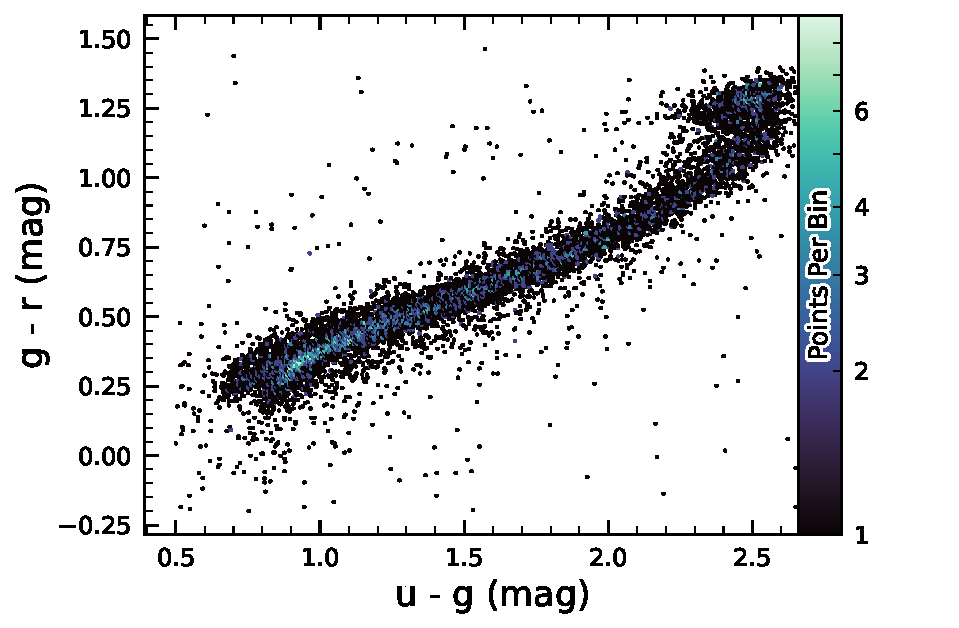
\includegraphics[width=\linewidth, height=5.8cm]{dp1_stellar_locus_ugr.pdf}
  \caption{$ugr$ stellar locus containing 12779 stars with signal-to-noise greater than 50 in the $u$ band.}
  \end{subfigure}\hfill
  \begin{subfigure}[t]{0.31\textwidth}
  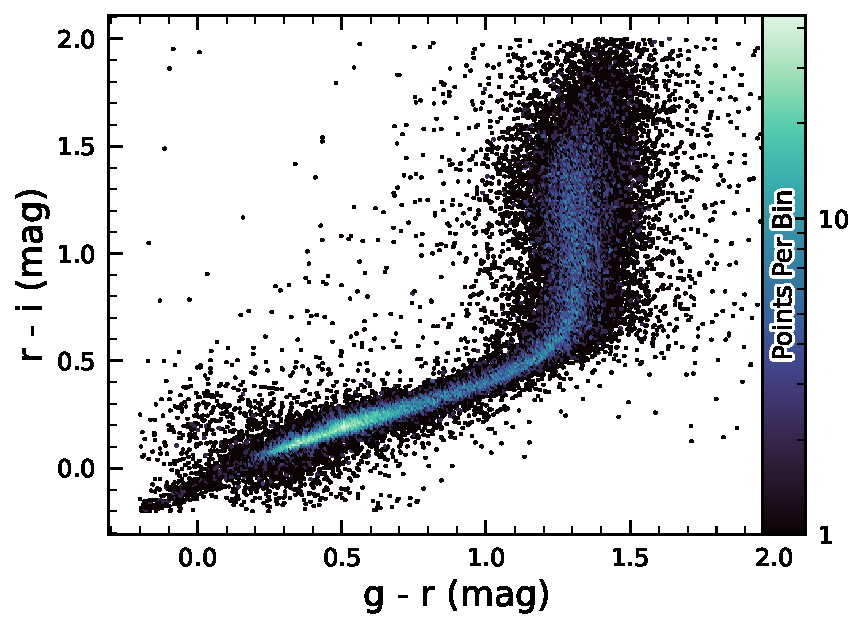
\includegraphics[width=\linewidth, height=5.8cm]{dp1_stellar_locus_gri.pdf}
  \caption{$gri$ stellar locus containing 63236 stars with signal-to-noise greater than 200 in the $i$ band.}
  \end{subfigure}\hfill
    \begin{subfigure}[t]{0.31\textwidth}
  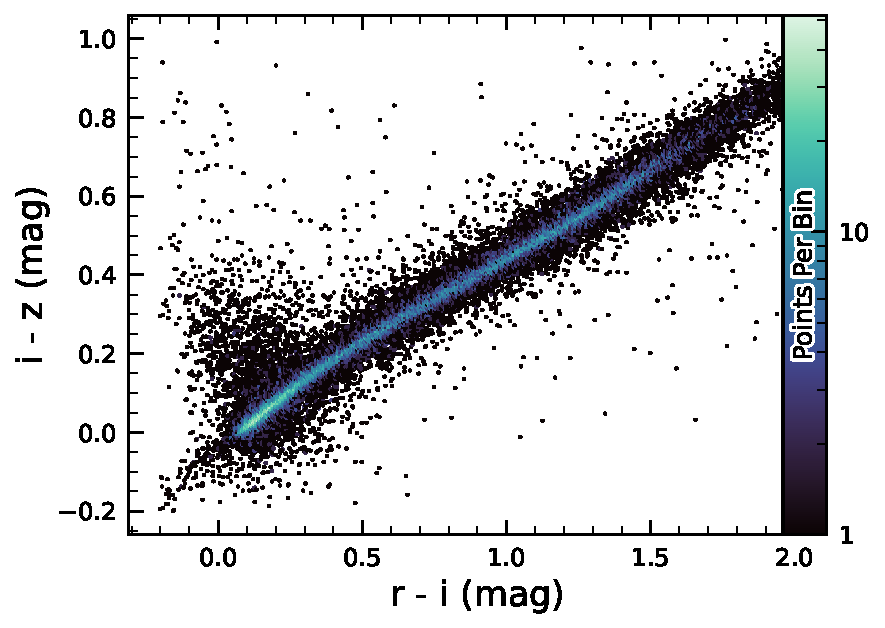
\includegraphics[width=\linewidth, height=5.8cm]{dp1_stellar_locus_riz.pdf}
  \caption{$riz$ stellar locus containing 46760 stars with signal-to-noise greater than 200 in the $i$ band.}
  \end{subfigure}\hfill
\caption{Examples of stellar loci from the full DP1 data set.}
  \label{fig:stellarloci}
\end{figure*}

%%
\subsection{Detection Completeness on Coadds}
\label{ssec:detection_completeness}
We characterize completeness by injecting synthetic sources into coadded images, and by comparing to external catalogs.
In both cases, we use a greedy, probabilistic matching \gls{algorithm}, whereby reference objects are matched in order of descending brightness to the most likely target within a $0.5''$ radius.

We inject sources in 12 of the patches of the \gls{ECDFS} region with the deepest coverage.
The input catalog contains stars and galaxies from part of the \gls{DC2} simulations \citep{2021ApJS..253...31L}, where the galaxies consist of an exponential disk and de Vaucouleurs \citep{1948AnAp...11..247D,1953MNRAS.113..134D} bulge.
To avoid deblender failures from excessive increases in object density, stars whose total \gls{flux} (i.e., summed across all six bands) is brighter than 17.5~${\rm mag_{\rm AB}}$ are excluded, as are galaxies whose total \gls{flux} is brighter than 15~${\rm mag_{AB}}$ or fainter than 26.5~${\rm mag_{AB}}$. Half of the remaining objects are selected for injection.

\begin{figure}[htb]
\centering
\includegraphics[width=0.98\linewidth]{figures/injected_lsst_cells_v1_5063_i_completeness_any.pdf}
\caption{Completeness as a function of $i$-band CModel magnitude for \gls{DC2}-based injections into a portion of the \gls{ECDFS} field.}
\label{fig:injected_lsst_cells_v1_5063_i_completeness_any}
\vspace{0.1cm}
\end{figure}

\figref{fig:injected_lsst_cells_v1_5063_i_completeness_any} shows completeness as a function of magnitude for these injected objects. The completeness estimates are comparable to results from matching external catalogs. The Hubble Legacy Field catalog \citep{2019ApJS..244...16W,2016arXiv160600841I} reaches 50\% completeness at 26.13\,${\rm mag_{F775W}}$, approximately 0.4 magnitudes fainter; this is roughly equivalent to 25.83\,${\rm mag_{i}}$ from differences in matched object magnitudes. Similarly, completeness drops below 90\% at 23.80${\rm mag_{VIS}}$ matching to Euclid Q1 \citep{2025arXiv250315305E} objects, equivalent to about 23.5\,${\rm mag_{i}}$. 
The Euclid imaging is of comparable or shallower depth, so magnitude limits at lower completeness percentages than 90\% are unreliable, whereas the HST images cover too small and irregular an area to accurately characterize 80-90\% completeness limits.
% DST: Is the above sentence TMI? It can be cut.

At the 80\% completeness limit, nearly 20\% of objects, primarily injected galaxies, are incorrectly classified as stars based on extendedness, which indicates whether a source is more likely to be a point source or an extended source.
Similarly, the fraction of correctly classified injected stars drops to about 50\% at 23.8\,${\rm mag_{i}}$ (90\% completeness).

There are several caveats for this analysis. The selection of objects for matching in any catalog is not trivial. Some fraction of the detections are either artifacts (particularly close to diffraction spikes around bright stars) or otherwise spurious. Additionally, some objects lie in masked regions of one survey but not another, which has not been accounted for. For injected source matching, the reference catalog does not include real on-sky objects. For this reason, we do not quote specific figures for purity; however, based on prior analyses of the \gls{DC2} simulations, purity is generally higher than completeness at any given magnitude.
% DST: The detection curve in DC2 is steeper and fainter than the equivalent source injection curve, despite DC2 having fewer visits. It's unclear whether this is due to (amongst other things) the relative simplicity of artifacts in DC2, differences in assumed filter response/gain, seeing distributions, etc. so this point is probably best left out.

\subsection{Flux Measurement}
\label{ssec:fluxes}

\begin{figure}[htb]
\centering
\includegraphics[width=0.98\linewidth]{figures/injected_lsst_cells_v1_5063_i_mag_cmodel.pdf}
\includegraphics[width=0.98\linewidth]{figures/injected_lsst_cells_v1_5063_i_mag_sersic.pdf}
\caption{Magnitude residuals for matched injected galaxies with the CModel and Sersic algorithms.}
\label{fig:injected_lsst_cells_v1_5063_i_mag}
\vspace{0.1cm}
\end{figure}

\figref{fig:injected_lsst_cells_v1_5063_i_mag} shows $i$-band magnitude residuals for CModel and Sersic measurements using the matched injected galaxies described in \secref{ssec:detection_completeness}.
Similar behavior is seen in other bands.
Sersic fluxes show reduced scatter and are more accurate on average for galaxies brighter than 22.5\,${\rm mag_{i}}$, though CModel's are less biased, with median residuals  slightly closer to zero.
For fainter objects, Sersic fluxes are more biased and less accurate.
The magnitude of this bias is considerably larger than previously seen in simulated data and is being investigated.
Aperture fluxes - including Kron and \gls{GAaP} - are not shown as they are not corrected to yield total fluxes and thus are not recommended for use as total galaxy magnitudes.

\begin{figure}[htb]
\centering
\includegraphics[width=0.98\linewidth]{figures/injected_lsst_cells_v1_5063_r_color_cmodel_g_minus_i.pdf}
\includegraphics[width=0.98\linewidth]{figures/injected_lsst_cells_v1_5063_r_color_gaap_g_minus_i.pdf}
\includegraphics[width=0.98\linewidth]{figures/injected_lsst_cells_v1_5063_r_color_sersic_g_minus_i.pdf}
\caption{$g-i$ color residuals versus injected r-band magnitude for matched galaxies with the CModel, \gls{GAaP} and Sersic algorithms.}
\label{fig:injected_lsst_cells_v1_5063_r_color_g_minus_i}
\vspace{0.1cm}
\end{figure}

\figref{fig:injected_lsst_cells_v1_5063_i_mag} shows $g-i$ color residuals versus $r$-band magnitude for the same sample of galaxies as \figref{fig:injected_lsst_cells_v1_5063_i_mag}.
For this and most other colors, \gls{GAaP} (with a $1''$ aperture) and Sersic colors both yield lower scatter; however, the CModel colors have the smallest bias.
Curiously, the \gls{GAaP} bias appears to be magnitude-dependent, whereas the Sersic bias remains stable from $19<r<26$.
Any of these color measurements are suitable for use for deriving quantities like photometric redshifts, stellar masses, etc.

In addition to photometry, some algorithms include measurements of structural parameters like size, ellipticity, and Sersic index.
One particular known issue is that many (truly) faint objects have significantly overestimated sizes and fluxes, as was also seen in the Dark Energy Survey \citep{2025arXiv250105739B}.
We dub such objects "super-spreaders".
These super-spreaders contribute significantly to overestimated fluxes at the faint end, and are particularly problematic for the Kron algorithm \citep{1980ApJS...43..305K}, which is not recommended for general use.

As mentioned in \secref{ssec:coadd_processing}, the Sersic fits include a free centroid, which is initialized from the fiducial centroid of the object.
Preliminary analyses of matched injected objects suggest that the galaxy \gls{astrometry} residuals are somewhat smaller, and so users of the Sersic photometry should also use these centroid values (if needed).
One caveat is that for faint objects and/or in crowded regions with unreliable deblending, free centroids can drift significantly and potentially towards other objects, so objects with large differences between the fiducial and Sersic \gls{astrometry} should be used with caution.

\subsection{Differential Chromatic Refraction}
%% This is an effect seen in ComCm - this section shows that but no correction is applied to proceessing in DP1.
%% Think we'll need to correct for this in templates  to some degree to prevent dipoles appearing as extrems color sources at hight airmass.
%% Science -- Fed -- measure stellar flar temperatures, AGN uise the effect to identiyf quasar lines - bight emmision lines in quasars as they transiotion.
\label{sec:differential_chromatic_refraction}
\gls{Differential Chromatic Refraction} (DCR) occurs when light passes through Earth’s atmosphere, refracting more for shorter wavelengths, which causes blue light to appear shifted closer to the zenith. 
This wavelength-dependent effect results in the smearing of point sources along the zenith direction, specifically parallel to the parallactic angle. 
The DCR effect is observable in LSSTComCam data, particularly in the angular offset versus g-i band magnitude difference plots,  as shown in \figref{fig:dcr}, which plots all direct sources with \gls{SNR} $>10$ from 41 visits from November 26, 2024. 
When looking at data perpendicular to the parallactic angle, sources show no DCR effect (as expected), forming a clear vertical distribution on the 2-dimensional density plots in \figref{fig:dcr}.

In contrast, sources aligned with the parallactic angle exhibit a tilted, linear distribution, clearly demonstrating the relationship between angular offset and the $g-i$ band magnitude difference, thereby providing a visual indication of the \gls{DCR} effect.

\begin{figure}[htb!]
\centering
\includegraphics[width=0.98\linewidth]{dcrHexbin.pdf}
\caption{Visualization of \gls{Differential Chromatic Refraction} (DCR) observed in the  LSSTComCam commissioning campaign. The $g-i$ color is computed for every source in the reference catalog that is matched to a direct source in the science image, and the binned density for the full survey is plotted against the angular offset between the reference and detected positions. The angular offset is projected along coordinates parallel and perpendicular to the parallactic angle of the observation, and shows a characteristic correlation along the parallel axis with no correlation along the perpendicular axis. The orange vertical dashed line indicates the expected $g-i$ magnitude distribution at zero angular offset, while the green ‘x’ marks the average $g-i$ magnitude of the plotted sources.}
\label{fig:dcr}
\vspace{0.1cm}
\end{figure}


% Eric
\subsection{Difference Imaging Purity} \label{sec:performance:dia}

We assessed the performance of image differencing using human vetting and source injection (\S \ref{sec:perf:dia_completeness}).
Members of the \gls{DP1} team labeled more than 9500 DIASource image triplets consisting of cutouts from the science, template, and difference images.
We classified these into various real and artifact categories.
The raw artifact to real ratio without filtering was roughly 9:1.
Bright stars are the main source of artifacts.
Correlated noise, primarily in u and g bands, also leads to spurious detections near the threshold.
We expect to be able to mitigate these effects for \gls{LSSTCam}.

Applying a reliability threshold improves the purity of transients but not variable stars; technical limitations at the time of model training prevented injection of variable stars into the synthetic training set.
Reliability models for \gls{LSSTCam} data will be trained on a wider range of input data.

\subsection{Detection Completeness on Difference Images} 
\label{sec:perf:dia_completeness}

We assess the performance of our difference imaging \gls{pipeline} using synthetic source injection on the science images prior to differencing.
We construct a catalog of injected sources by joining two different samples of point sources, a set of hosted sources to emulate transients in galaxies and second set of hostless sources.

The hosts are selected from the \gls{pipeline} source catalog that is produced upstream by imposing a cut in their extendedness measurement, and selecting $N_{\rm src}={\rm min}(100, N\times0.05)$ of the available sources per detector.
%
% filtered_sources = sources[(sources['extendedness'] == 1) & (sources['sizeExtendedness']>0.90) & (sources['calibFlux'] > 0)]
%
For each host we pick a random position angle and radius using its light profile \gls{shape}, and also a random value of brightness for the injected source, with magnitudes higher than the host source.
The hostless sources instead have random positions in the \gls{CCD} focal plane, and with magnitudes chosen from a random uniform distribution with $20 \geq m \geq m_{lim} + 1$  with $m_{lim}$ the limiting magnitude of the image.

We used the \gls{LSST} package \texttt{source\_injection} to include these sources into our test images, we performed a coordinate cross-match task, with a threshold of $0.''5$ to find which of these sources were detected and which were lost, enabling the calculation of a set of performance metrics.
%These include i) the detection completeness as function of signal to noise ratio (S/N), ii) the distribution of the coordinate offsets for the found sources, both in sky coordinates and focal plane coordinates, iii) the flux pull distribution both of PSF photometry measurements as well as aperture measurements, iv) the spatial correlation of the positions of both the found and missed sources, in sky coordinates and focal plane coordinates, v) the magnitude and S/N dependency of the astrometry and photometry recovery for the found sources, vi) the detection efficiency as function of the distance and brightness of the host, and vii) the reliability score of the synthetic sources.
%For all of these listed metrics we find results consistent with our expected parameters and required tolerances.

In \figref{fig:eff_snr_griz} we show the detection completeness as function of the \gls{SNR}, for sources in the \gls{ECDFS} field, for filters \textit{griz}. We observe a completeness $>95\%$ for sources with \gls{SNR}$> 6$, with mean completeness $\simeq 99\%$ and standard deviation of $\simeq 0.7\%$.
%
\begin{figure}[htb!]
\centering
\includegraphics[width=0.98\linewidth]{figures/efficiency_snr_griz.pdf}
\caption{The difference image detection completeness for injected sources in the \gls{ECDFS} field, for filters \textit{griz}, as function of the estimated signal to noise ratio S/N. This completeness is the ratio between the found fake sources (shaded histogram) and all the sources (solid line). The horizontal dashed line represents where the $50\%$ completeness level is reached, at approximately S/N $\simeq 5.07$.}
\label{fig:eff_snr_griz}
\vspace{0.1cm}
\end{figure}
%
In \figref{fig:coordinate_offset_diffim_fakes} we show the distribution of the residuals of the recovered sky coordinates for the detected synthetic sources. The marginal distributions are both centered at zero, and they are compatible with normal distributions $\mathcal{N}(0, 0''.04)$.
%
\begin{figure}[htb!]
\centering
\includegraphics[trim={0 0 0 0},width=\linewidth]{figures/coordinate_offsets_hexbin.pdf}
\caption{Coordinate residuals for detected synthetic sources in difference images, between recovered and true position of the sources in the \gls{ECDFS} field. In the top and right panels we include the histogram of these offsets. The circle reflects the matching radius of $0''.5$.}
\label{fig:coordinate_offset_diffim_fakes}
\end{figure}
%
In \figref{fig:phot_residual_diffim_fakes} we show the recovered magnitudes for our detected synthetic sources in the \textit{i} filter, using \gls{PSF} photometry on the difference images, and also show marginal distributions of the true magnitudes for fake sources, and the residuals on the left, split into hosted and hostless.
%
Our \gls{flux} measurements are accurate within a wide range of magnitudes, for both hosted and hostless synthetic sources. 
For true $m_i < 22.2$, the median PSF magnitudes residuals are $<0.1$. 
When considering the \gls{flux} pulls $\delta = (f-f_{\rm{True}})/\sigma_f$ for PSF \gls{flux} $f$ and error $\sigma_f$, we find that $|\left<\delta\right>| <0.1$, and $\sigma_\delta < 1.1$ for $m_i<21.6$.
%
\begin{figure}
    \centering
    \includegraphics[width=\linewidth]{figures/hexbin_psf_mag.pdf}
    \caption{Magnitude residuals for \gls{PSF} photometry on difference images for ECDFS field in $i$ for detected fake sources. In black solid and dashed lines: the running median, and the mean absolute deviation. Top panel: the distribution of true magnitudes for hostless and hosted fakes sources. Right panel: the distribution of magnitude residuals for hostless and hosted sources.}
    \label{fig:phot_residual_diffim_fakes}
\end{figure}

% Jake/Mario
\subsection{Solar System}
\label{sec:performance:solsys}

\subsubsection{Asteroid Linking Performance}

\gls{DP1} performance evaluation of asteroid linking focused on demonstrating discovery capability.
The solar system discovery \gls{pipeline} produced 269,581 tracklets, 5,691 linkages, and 281 post-processed candidates.

We performed a conservative manual investigation of these 281 candidates, producing a curated list of \nnewasteroiddiscoveries probable new asteroid discoveries.
All of these candidates are identified as main-belt asteroids.
As described in Section~\ref{sec:drp:solsys}, post processing of the {\tt heliolinc} output with {\tt link\_purify} produced a final set of 281 candidate linkages, ranked with the most promising candidates first.
Using {\tt find\_orb} \citep{findorb}, we derived orbit fits for each candidate, sorting the resulting list by $\chi_{\rm dof}^2$, the quality of the fit.
Manual inspection of the linkages indicated that those ranked 0--137 corresponded to unique real asteroids; ranks 138--200 contained additional real objects intermixed with some spurious linkages; an d ranks higher than 200 were essentially all spurious.
This analysis indicates that it will be possible to identify cuts on quality metrics like $\chi^2$ to derive discovery candidate samples with high purity; determining the exact quantitative cut values requires more data with \gls{LSSTCam}.
We next removed all observations matched to known asteroids (using \gls{MPC}'s MPChecker service), reducing the number of candidates to 97.
Of these, four had strong astrometric and/or photometric outliers, likely due to self-subtraction in difference images due to the unavoidable limitations of template generation from the limited quantity of data available from  \gls{LSSTComCam}.
We suspect these four linkages do correspond to real objects, but have chosen to discard them out of an abundance of caution.
The remaining \nnewasteroiddiscoveries were submitted to the Minor Planet Center and accepted as new discoveries, demonstrating the \gls{LSST} pipelines are able to successfully discover new solar system objects.
%\jake{We should cite the MPEC with discoveries, once we do submit and the MPEC becomes available}

\subsubsection{Asteroid Association Performance}

Solar system association associated \nsolarsystemsources DiaSources to \nsolarsystemobjects unique solar system objects. 
%\jake{Update this after table update!}
These include 3,934 DiaSources to 338 already-known \gls{MPC} objects and 2,054 DiaSources to the \nnewasteroiddiscoveries  newly-discovered objects.
Association also picked up an additional 143 detections of newly discovered objects.
% \jake{This too - new parameter in notebook.}
These were not originally found by the discovery pipelines as they didn't satisfy the number and/or maximum time span requirements to form tracklets.

\begin{figure}[htb!]
\centering
\includegraphics[width=0.98\linewidth]{figures/sso_residuals.pdf}
\caption{Astrometric residuals between expected and observed positions of SSOs in \gls{DP1}. The median residuals are $0.''001$ and $-0.''016$ in R.A./Dec direction, with the standard deviations of $0.''19$ and $0.''10$, respectively. No detectable detectable systematic offset from zero indicates there are no major errors in either timing or astrometry delivered by the Rubin system. The wider scatter in the RA-direction is due to objects whose measured orbital elements are less well constrained, translating to larger along-track positional errors in the predicted positions.}
\label{fig:sso_residuals}
\vspace{0.1cm}
\end{figure}

The astrometric residuals of known asteroid association are shown in Figure \ref{fig:sso_residuals}. 
%\jake{Todo:} 
Astrometric precision for solar system sources is excellent, the majority of objects detected within $0''.1$ of their expected positions. 
Taking the unsigned median residuals to search for biases, we find that previously-known objects have mean residuals of $0.''001$ and $-0.''016$ in the \gls{RA} and Dec directions respectively, while newly-discovered objects have mean residuals of $-0.''035$ and $-0.''010$ in the \gls{RA} and Dec directions, respectively. 
These mean residuals are small enough to eliminate the possibility of a timing offset greater than the second-scale shutter motion (which is uncharacterized for LSSTComCam).

\subsection{Crowded Fields}
Two of the seven \gls{DP1} target fields exhibit high stellar density, 47 Tucanae and the Fornax dwarf galaxy.
47 Tucanae was chosen as an initial stress test for the science pipelines processing.
The Fornax dwarf galaxy also exhibits high stellar density, particularly in its central regions.
%\yusra{Explain where the pipelines broke down. and  how the performance is different in the 2 crowded fields}

% Lead: Leanne, Reviewed by Gregory, Wil, Adam.
\section{Rubin Science Platform}
\label{sec:data_services}

The \gls{RSP} \citep{LSE-319} is a powerful, cloud-based environment for scientific research and analysis of petascale-scale astronomical survey data.
It serves as the primary interface for scientists to access, visualize, and conduct next-to-the-data analysis of Rubin and \gls{LSST} data.
The  \gls{RSP} is designed around a  ``bring the compute to the data'' principle, eliminating the need for users to download massive datasets.
Although \gls{DP1} is comparable in size (\sizeinbytes) to existing survey datasets, future \gls{LSST} datasets will be larger and more complex, making it crucial to co-locate data and analysis for effective scientific discovery.

The \gls{RSP} provides users with access to data and services through three distinct user-facing Aspects: a \emph{Portal}, which facilitates interactive exploration of the data; a JupyterLab-based \emph{Notebook} environment for data analysis using Python; and an extensive set of \emph{\glspl{API}} that enable programmatic access to both data and services.
The three Aspects are designed to be fully integrated, enabling seamless workflows across the \gls{RSP}.
The data products described in \secref{sec:data_products} are accessible via all three Aspects, and the system facilitates operations such as starting a query in one Aspect and retrieving its results in another.
\figref{fig:rsp_landing_page} shows the Rubin \gls{Science Platform} landing page in the Google cloud.
\begin{figure}[htb!]
\centering
\includegraphics[width=0.98\linewidth]{data_access/rsp_landing_page.png}
\caption{The Rubin \gls{Science Platform} landing page showing the thress Aspects as well as links to documentation and support information.}
\label{fig:rsp_landing_page}
\vspace{0.1cm}
\end{figure}

The \gls{RSP} is supported by a number of back-end services, including databases, files, and batch computing.
Support for collaborative work through shared workspaces is also included in the \gls{RSP}.

A preview of the \gls{RSP} was launched on Google Cloud in 2022, operating under a shared-risk model to support \href{https://dp0.lsst.io/}{Data Preview 0} \citep{2024ASPC..535..227O}. This allowed the community to test the platform, begin preparations  for science, and provide valuable feedback to inform ongoing development.
It was the first time an astronomical research environment was hosted in a \gls{cloud} environment.
The DP1 release brings major updates to \gls{RSP} services, enhancing scientific analysis capabilities.
The \gls{RSP} remains under active development, with incremental improvements being rolled out as they mature.
During the Rubin Early Science Phase, the \gls{RSP} will continue to operate under a shared-risk model.
This section outlines the RSP functionality available at the time of the DP1 release and provides an overview of planned future capabilities.

% Section reviewed by Adam
\subsection{Rubin Data Access Center
\label{ssec:usdac}}
The Rubin USDAC utilizes a novel hybrid on-premises-\gls{cloud} architecture, which combines on-premises infrastructure at the \gls{USDF} at SLAC with flexible and scalable resources in the Google \gls{cloud}.
This architecture has been deployed and tested using the larger simulated data set of DP0.2 \citep{2024SPIE13101E..2BO}.

In this hybrid model, user-facing services are deployed in the \gls{cloud} to support
dynamic scaling in response to user demand and to simplify the provisioning and management of large numbers of science user accounts.
The majority of the static data products described in \secref{sec:data_products} are stored on-premises at the \gls{USDF} to benefit from cost-effective mass storage and close integration with Rubin data processing infrastructure, also located at the \gls{USDF}.
For imaging data, the Data Butler (\secref{sssec:data_butler}) provides the interface between the \gls{cloud}-based users and data services, and the on-premises data.
For catalog data, a \gls{cloud}-based \gls{TAP} client (\secref{sssec:ivoa_services}) submits queries to the on-premises \gls{Qserv} database cluster (\secref{ssec:databases}) and retrieves the results.
In the initial DP1 deployment, catalog data is hosted at the \gls{USDF} while image data is stored in the cloud.
The full hybrid model will be rolled out and further tested following the release of \gls{DP1}.

The RSP features a single-sign-on authentication and authorization system to provide secure access for Rubin data rights holders \citep{rdo-013}

\subsection{API Aspect
\label{ssec:rsp_api}}
The \gls{API} Aspect provides a comprehensive set of user-facing interfaces for programmatic access to the \gls{DP1} data products, through both \gls{IVOA}-compliant services and the Rubin Data Butler. IVOA services enable standard queries and integration with existing tools, while the Butler facilitates advanced data processing within the \gls{LSST Science Pipelines}.

At the time of the \gls{DP1} release, some \gls{IVOA} services are unavailable, and certain data products are only accessible via the Butler.
This section provides an overview of the available \gls{IVOA} services and Butler access.

% IVOA services
\subsubsection{IVOA Services
\label{sssec:ivoa_services}}

Rubin has adopted a \gls{VO}-first design philosophy, prioritizing compliance with \gls{IVOA} standard interfaces to foster interoperability, standardization, and collaboration.
In cases where standardized protocols have yet to be established, additional services have been introduced to complement these efforts.
This approach ensures that the RSP can be seamlessly integrated with community-standard tools such as TOPCAT \citep{2011ascl.soft01010T} and Aladin \citep{2000A&AS..143...33B, 2014ASPC..485..277B, 2022ASPC..532....7B}, as well as libraries such as  PyVO \citep{2014ascl.soft02004G}.

The user-facing \glspl{API} are also used internally within the \gls{RSP}, creating a unified design that ensures consistent and reproducible workflows across all three Aspects.
This reduces code duplication, simplifies maintenance, and ensures all users, both internal and external, access data in the same way.
For example, an \gls{ADQL} query on the \gls{Object} catalog via TAP yields identical results whether run from the Portal, Notebook, or an external client.

The following \gls{IVOA} services are available at the time of the DP1 release:
\begin{itemize}
\vspace{0.1cm}
\item \textbf{Table Access Protocol (TAP) Service}: A TAP service \citep{2019ivoa.spec.0927D} enables queries of catalog data via the IVOA-standard \gls{ADQL}, a dialect of SQL92 with spherical geometry extensions.
The main \gls{TAP} service for \gls{DP1} runs on the Rubin-developed \gls{Qserv} database (\S~\ref{ssec:databases}), which hosts the core science tables described in \secref{ssec:catalogs}, as well as the Visit database.
It also provides image metadata in the IVOA ObsCore format via the standard \texttt{ivoa.ObsCore} table, making it an ``ObsTAP'' service \citep[ObsTAP;][]{2017ivoa.spec.0509L}.
The TAP service is based on the \gls{CADC}'s open-source Java TAP implementation\footnote{https://github.com/opencadc/tap}, modified for the exact query language accepted by Qserv.
It currently supports a large subset of ADQL, with limitations documented in the data release materials (see \secref{ssec:documentation}) and exposed via the TAP \textbf{capabilities} endpoint where possible. \

The TAP service provides metadata annotations consistent with the standard, including table and column descriptions, indications of foreign-key relationships between tables, and column metadata such as units and \gls{IVOA} Unified Content Descriptors (UCDs).

% Image Services
\vspace{0.1cm}
\item \textbf{Image Access Services}: Rubin image access services are compliant with \gls{IVOA} SIAv2 \citep[Simple Image Access Protocol, version 2;][]{2025arXiv250100544J,2015ivoa.spec.1223D}
for discovering and accessing astronomical images based on \gls{metadata}.
For example, querying for all images in a given band over a particular sky region observed during a given period.
SIAv2 is a \gls{REST}-based protocol that supports the discovery and retrieval of image data.
%e.g. \url{https://<rubin-sia-service-url>?POS=180.0,0.0&SIZE=0.01}
Users identify an image or observation of interest and query the service.
The result set includes \gls{metadata} about the image, such as the sky position, time, or band, and a data access URL, which includes an IVOA Identifier uniquely identifying the dataset \citep{DMTN-302}, allowing the dataset to be retrieved or a cutout requested via \gls{SODA}.

% Image cutout services
\vspace{0.1cm}
\item \textbf{Image Cutout Service}: The Rubin Cutout Service \citep{SQR-063, SQR-093} is based on the  \gls{IVOA} SODA \citep[Server-side Operations for Data Access;][]{2017ivoa.spec.0517B}.
Users submit requests specifying sky coordinates and the cutout size as the radius from the coordinates, and the  service performs the operation on the full image and returns a result set.
% For a YxY cutout, the typical size of the returned result set is <X>
For \gls{DP1}, The  cutout service is a single cutout service only where N cutout requests will require N independent synchronous calls.
We expect some form of bulk cutout service by mid 2026, approximately contemporaneously with \gls{DP2}

% HIPS
\vspace{0.1cm}
\item \textbf{HiPS Data Service}: An authenticated \gls{HiPS}
%\footnote{HiPS is an IVOA standard for multi-resolution tiled image data.}
\citep{2017ivoa.spec.0519F}
%\citep[Hierarchical Progressive Surveys;][]{2017ivoa.spec.0519F}
data service for seamless pan-and-zoom access to large-scale co-adds.
It supports fast interactive progressive image exploration at a range of resolutions.

% WebDAV
\vspace{0.1cm}
\item \textbf{WebDAV}: A \gls{WebDav} service is provided to enable users to remotely manage, edit, and organize files and directories on the \gls{RSP} as if they were local files on their own computer. This is especially useful for local development.
\end{itemize}

%%%%% Data Butler
\subsubsection{Data Butler
\label{sssec:data_butler}}

The Rubin Data Butler \citep{2022SPIE12189E..11J,2023arXiv230303313L},  is a high-level interface designed to facilitate seamless access to data for both users and software systems.
This includes managing storage formats, physical locations, data staging, and database mappings.
A \gls{Butler} repository contains two components:
\begin{itemize}
    \item the \emph{Data Store}: A physical storage system for datasets, e.g., a \gls{POSIX} file system or S3 object store; and
    \item the \emph{Registry}: An \gls{SQL}-compatible database that stores metadata about the datasets in the data store, see \secref{sssec:butler_registry}.
\end{itemize}
% Current plan is for DP1 image data to be cloud-hosted for the initial release and then transition to USDF back-end once we get through the initial surge.
For DP1, the Butler repository is hosted in the Google Cloud, using an \gls{S3}-compatible store for datasets and AlloyDB, a PostgreSQL-compatible database, for the registry.

In the context of the \gls{Butler}, a \emph{dataset} refers to a unique data product, such as an image, catalog or map, generated by the observatory or processing pipelines
Datasets belong to one of the various types of data products, described in \secref{sec:data_products}.
The \gls{Butler} ensures that each dataset is uniquely identifiable by a combination of three pieces of information: a data coordinate, a dataset type, and a run collection.
For example, a dataset that represents a single raw image with detector 8 during the on-sky campaign on the night starting 2024-11-11 in the $i$ band with exposure ID 2024111100074 would be represented as  \texttt{dataId={'exposure':2024111100074, 'band':'i', 'instrument':'LSSTComCam'}} and is associated with the \texttt{raw} DatasetType.
For a deep coadd on a \gls{patch} of sky in the Seagull field, there would be no exposure dimensions and would instead the tract, \gls{patch} and band would be specified as  \texttt{dataId={'tract':7850, 'patch': 6, 'band':'g', 'instrument':'LSSTComCam', skymap='lsst\_cells\_v1'}} and is associated with the \texttt{deep\_coadd} DatasetType.

\begin{deluxetable}{lcc}
\tablecaption{Simple Test Table\label{tab:dp1_dimensions}}
\tablehead{
  \colhead{Dimension} & 
  \colhead{Format/Valid values} & 
  \colhead{Description}
}
\startdata
\texttt{day\_obs} & YYYYMMDD & A day and night of observations that rolls over during daylight hours.\\
\texttt{visit} & YYYYMMDD\#\#\#\#\# & A sequence of observations processed together; synonymous with ``exposure'' in DP1.\\
\texttt{exposure} & YYYYMMDD\#\#\#\#\# & A single exposure of all nine ComCam detectors.\\
\texttt{instrument} & LSSTComCam & The instrument name.\\
\texttt{detector} & 0--8 & A ComCam detector.\\
\texttt{skymap} & \texttt{lsst\_cells\_v1} & A set of tracts and patches that subdivide the sky into rectangular regions with simple projections and intentional overlaps.\\
\texttt{tract} & See \tabref{tab:dp1_tracts} & A large rectangular region of the sky.\\
\texttt{patch} & 0--99 & A rectangular region within a tract.\\
\texttt{physical\_filter} & u\_02, g\_01, i\_06, r\_03, z\_03, y\_04 & An astronomical filter.\\
\texttt{band} & u, g, r, i, z, y & An astronomical wave band.
\enddata
\end{deluxetable}
%%%%% This table is auto generated from data, DO NOT EDIT
%\begin{deluxetable}{lp{3.5cm}p{8cm}}
%\tablecaption{Descriptions of and valid values for the key data dimensions in DP1. YYYYMMDD signifies date and \# signifies a single 0--9 digit.
%\label{tab:dp1_dimensions}}
%\tablehead{
%  \colhead{\textbf{Dimension}} &
%  \colhead{\textbf{Format/Valid values}} & 
%  \colhead{\textbf{Description}}\\
%}
%\startdata
%\texttt{day\_obs} & YYYYMMDD & A day and night of observations that rolls over during daylight hours.\\
%\texttt{visit} & YYYYMMDD\#\#\#\#\# & A sequence of observations processed together; synonymous with ``exposure'' in DP1.\\
%\texttt{exposure} & YYYYMMDD\#\#\#\#\# & A single exposure of all nine ComCam detectors.\\
%\texttt{instrument} & LSSTComCam & The instrument name.\\
%\texttt{detector} & 0--8 & A ComCam detector.\\
%\texttt{skymap} & \texttt{lsst\_cells\_v1} & A set of tracts and patches that subdivide the sky into rectangular regions with simple projections and intentional overlaps.\\
%\texttt{tract} & See \tabref{tab:dp1_tracts} & A large rectangular region of the sky.\\
%\texttt{patch} & 0--99 & A rectangular region within a tract.\\
%\texttt{physical\_filter} & u\_02, g\_01, i\_06, r\_03, z\_03, y\_04 & An astronomical filter.\\
%\texttt{band} & u, g, r, i, z, y & An astronomical wave band.
%\enddata
%\end{deluxetable}

The data coordinate is used to locate a dataset in multi-dimensional space, where dimensions are defined in terms of scientifically meaningful concepts, such as instrument, visit, detector or band.
For example, a calibrated single-visit image (\secref{ssec:science_images}) has dimensions including band, instrument, and detector.
In contrast, the visit table (\secref{ssec:catalogs}), a catalog of all calibrated single-epoch visits in \gls{DP1}, has only the instrument dimension.
The main dimensions used in \gls{DP1} are listed, together with a brief description, in \tabref{tab:dp1_dimensions}.
To determine which dimensions are relevant for a specific dataset, the \gls{Butler} defines dataset types, which associate each dataset with its specific set of relevant dimensions, as well as the associated Python type representing the dataset.
The dataset type defines the kind of data a dataset represents.
For example, a raw image  (\texttt{raw}), a processed catalog (\texttt{object\_forced\_source}), or a \gls{sky map} (\texttt{skyMap}).

\tabref{tab:butlerdatasets} lists all the dataset types available via the Butler in DP1, together with the dimensions needed to uniquely identify a specific dataset and the number of unique datasets of each type. It is important to highlight a key difference between accessing catalog data via the \gls{TAP} service versus the Butler. While the \gls{TAP} service contains entire catalogs, many of the same catalogs in the Butler are split into multiple separate catalogs. This is partly due to how these catalogs are generated, but also because of the way data is stored within and retrieved from the Butler repository -- it is inefficient to retrieve the entire \texttt{Source} catalog, for example, from the file system. Instead, because the \texttt{Source} catalog contains data for sources detected in the \texttt{visit\_image}s, there is one \texttt{Source} catalog in the Butler for each \texttt{visit\_image}. Similarly, there is one \texttt{Object} catalog for each \texttt{deep\_coadd}. All the catalogs described in \secref{ssec:catalogs}, aside from the \texttt{CcdVisit}, \texttt{SSObject}, \texttt{SSSource}, and \texttt{Calibration} catalogs, are split within the Butler.

%%%%% This table is auto generated from data, DO NOT EDIT
\setlength{\tabcolsep}{6pt}  % default is 6pt
\begin{deluxetable}{llcc}
\tablecaption{The name and number of each type of data product in the Butler and the dimensions required to identify a specific dataset.
\label{tab:butlerdatasets} }

\tablehead{
  \textbf{Data Product} & 
  \textbf{Name in Butler} & 
  \textbf{Required Dimensions} & 
  \textbf{Number in DP1}\
}
\startdata
\texttt{raw}&\texttt{raw}&instrument, detector, exposure&16125\\
\texttt{visit\_image}&\texttt{visit\_image}&instrument, detector, visit&15972\\
\texttt{deep\_coadd}&\texttt{deep\_coadd}&band, skymap, tract, patch&2644\\
\texttt{template\_coadd}&\texttt{template\_coadd}&band, skymap, tract, patch&2730\\
\texttt{difference\_image}&\texttt{difference\_image}&instrument, detector, visit&15972\\
\texttt{Source}&\texttt{source}&instrument, visit&1786\\
\texttt{Object}&\texttt{object}&skymap, tract&29\\
\texttt{ForcedSource}&\texttt{object\_forced\_source}&skymap, tract, patch&636\\
\texttt{DiaSource}&\texttt{dia\_source}&skymap, tract&25\\
\texttt{DiaObject}&\texttt{dia\_object}&skymap, tract&25\\
\texttt{ForcedSourceOnDiaObject}&\texttt{dia\_object\_forced\_source}&skymap, tract, patch&597\\
\texttt{CCDVisit}&\texttt{visit\_detector\_table}&instrument&1\\
\texttt{SSObject}&\texttt{ss\_object}&--&1\\
\texttt{SSSource}&\texttt{ss\_source}&--&1\\
\texttt{Visit}&\texttt{visit\_table}&instrument&1\\
\enddata
\end{deluxetable}


A dataset is associated with one or more \emph{Run Collections}; logical groupings of  datasets within the \gls{Butler} system that were created or processed together by the same batch operation.
Collections allow multiple datasets with the same data coordinate to coexist without conflict.
Run Collections support flexible, parallel processing by enabling repeated analyses of the same input data using different configurations.

For \gls{DP1}, a subset of the consolidated database contents (\secref{sssec:consdb}) is accessible through the Data Butler. However, not all metadata from the \texttt{Visit} table (\secref{ssec:metadata}) is available.
The \gls{DP1} Butler is read-only; a writeable Butler is expected by mid-2026, around the time of \gls{DP2}.

\subsubsection{Remote Programmatic Access
\label{sssec:remote_api}}
The Rubin \gls{RSP} \gls{API} can be accessed from a local system by data rights holders outside of the \gls{RSP}, by creating a user security token. This token can then be used as a bearer token for \gls{API} calls to the \gls{RSP} TAP service.
This capability is especially useful for remote data analysis using tools such as \gls{TOPCAT}, as well as enabling third-party systems (e.g., Community Alert Brokers) to access Rubin data. Additionally, it supports remote development with local IDEs, allowing for more flexible workflows and integration with external systems.

% Portal
\subsection{Portal Aspect
\label{ssec:rsp_portal}}
The Portal Aspect provides an interactive environment for exploratory data discovery, query, filtering, and visualization of both image and catalog data,  without requiring programming experience.

It enables users to search, visualize, and interact with large datasets through tools for catalog queries, image browsing, time series inspection, and cross-matching.
The Portal is designed to support both exploratory data access and detailed scientific investigation.

The Portal is built on \gls{Firefly} \citep{2019ASPC..521...32W}, a powerful web application framework developed by IPAC (Infrared Processing and Analysis Center).
\gls{Firefly} provides interactive capabilities such as customizable table views, image overlays, multi-panel visualizations, and linked displays between catalogs and images.
Through \gls{Firefly}, the Portal delivers a responsive and intuitive user experience, allowing users to analyze data visually while maintaining access to underlying metadata and query controls.
\begin{figure}[htb]
\centering
\includegraphics[width=0.98\linewidth]{data_access/rsp_portal_light.png}
\caption{The Rubin \gls{Science Platform} Portal Aspect}
% \gregory{Replace with a real DP1 image}
\label{fig:rsp_portal}
\end{figure}

\subsection{Notebook Aspect
\label{subsec:notebook}}
The Notebook Aspect provides an interactive, web-based environment built on Jupyter Notebooks, enabling users to write and execute Python code directly on Rubin and \gls{LSST} data without downloading it locally.
It offers programmatic access to Rubin and LSST data products, allowing users to query and retrieve datasets, manipulate and display images, compute derived properties, plot results, and reprocess data using the \gls{LSST Science Pipelines} (\secref{ssec:pipelines}).
The environment comes pre-installed with the pipelines and a broad set of widely used astronomical \gls{software} tools, supporting immediate and flexible data analysis.

\subsection{Databases
\label{ssec:databases}}
The user-facing Aspects of the \gls{RSP} are supported by several backend databases that store catalog data products, image metadata, and other derived datasets.
The \gls{schema} for DP1 and other Rubin databases is available online at \url{https://sdm-schemas.lsst.io}.

% Qserv -- Done
% Reviewed and approved by Fritz M.
% DP1 qserv catalog data will be hosted from SLAC from day 1.
\subsubsection{Qserv
\label{sssec:qserv}}
The final 10-year \gls{LSST} catalog is expected to reach \tenyearcatalogsize and contain measurements for billions of stars and galaxies across trillions of detections.
To support efficient storage, querying, and analysis of this dataset,  Rubin Observatory developed Qserv \citep{Wang:2011:QDS:2063348.2063364, C15_adassxxxii} -- a scalable, parallel, distributed SQL database system.
\gls{Qserv} partitions data over approximately equal-area regions of the celestial sphere, replicates data to ensure resilience and high availability, and uses shared scanning to reduce overall I/O load.
It also supports a package of scientific user-defined functions (SciSQL: \url{https://smonkewitz.github.io/scisql/}) simplifying complex queries involving spherical geometry, statistics, and photometry.
\gls{Qserv} is built on robust production-quality components, including MariaDB (\url{https://www.mariadb.org/}) and XRootD (\url{https://xrootd.org/}).
Qserv runs at the \gls{USDF} and user access to catalog data is via the TAP service (\secref{sssec:ivoa_services}).
This enables catalog-based analysis through both the \gls{RSP} Portal and Notebook Aspects.

Although the small \gls{DP1} dataset does not require Qserv’s full capabilities, we nevertheless chose to use it for \gls{DP1} to accurately reflect the future data access environment and to gain experience with scientifically-motivated queries ahead of full-scale deployment.
\gls{Qserv} is open-source and available on GitHub: \url{https://github.com/lsst/qserv}.

% is this needed?
\subsubsection{Butler Registry
\label{sssec:butler_registry}}
The \gls{Butler} registry is a relational database that manages metadata and relationships between the various datasets in a data preview or release.
For \gls{DP1}, the registry is hosted on Google using AlloyDB, a PostgreSQL-compatible database.

% Reviewed by Wil, Fritz , KT, GPDF
\subsubsection{Consolidated Database
\label{sssec:consdb}}

The Consolidated Database (ConsDB) \citep{dmtn-227} is an SQL-compatible database designed to store and manage metadata for Rubin Observatory science and calibration images.
Metadata is recorded on a per-exposure basis and includes information such as the target name, pointing coordinates, observation time, physical filter and band, exposure duration, and environmental conditions (e.g., temperature, humidity, and wind speed).
This key image metadata is also stored in the Butler Registry (\secref{sssec:data_butler}), however the ConsDB stores additional information  including derived metrics from image processing and information from the \gls{EFD} transformed from the time dimension to the exposure dimension.

The ConsDB schema is organized into instrument-specific tables, e.g., \gls{LSSTComCam} and LSSTCam, facilitating instrument-specific queries.
Within the \gls{LSSTComCam} schema, data is further structured into tables for individual exposures and detectors.
An example query on the \gls{DP1} dataset might retrieve all visits within a specified time range in the r-band for a given \gls{DP1} target.

The ConsDB is hosted at the \gls{USDF}.
Following the initial release of DP1, a release of the DP1 exposure-specific ConsDB data will be made available through the \gls{RSP}, and accessible externally via TAP.
The detailed \gls{LSSTComCam} schema can be found at:
\url{https://sdm-schemas.lsst.io/cdb_lsstcomcam.html}

% Lead Melissa, reviewed by Leanne
\section{Support for Community Science
\label{sec:community_science}}

The Rubin Observatory has a science community that encompasses thousands of individuals worldwide, with a broad range of experience and expertise in astronomy in general, and in the analysis of optical imaging data specifically.

Rubin's model to support this diverse community to access and analyze \gls{DP1} emphasizes self-help via documentation and tutorials, and employs an open platform for asynchronous issue reporting that enables crowd-sourced solutions.
These two aspects of community support are augmented by virtual engagement activities.
In addition, Rubin supports its Users Committee to advocate on behalf of the science community, and supports the eight \gls{LSST} Science Collaborations.

All of the resources for scientists that are discussed in this section are discoverable by browsing the For Scientists pages of the Rubin Observatory website\footnote{\url{https://rubinobservatory.org/}}.

\subsection{Documentation
\label{ssec:documentation}}

The data release documentation for \gls{DP1} can be found at \url{dp1.lsst.io}.
The contents include an overview of the \gls{LSSTComCam} observations, descriptions of the data products (images and catalogs), and a high-level summary of the processing pipelines.
Similar to the contents of this paper, but presented in a browsable, searchable webpage built with Sphinx\footnote{\url{https://www.sphinx-doc.org/}}, and written with a focus on applications of the data products to scientific analysis.

\subsection{Tutorials
\label{ssec:tutorials}}

A suite of tutorials that demonstrate how to access and analyze \gls{DP1} using the RSP accompany the data release.
Jupyter Notebook tutorials are available via the ``Tutorials'' drop-down menu within the Notebook aspect of the \gls{RSP}.
Tutorials for the Portal and API aspects of the \gls{RSP} can be found in the data release documentation.

These tutorials are designed to be inclusive, accessible, clear, focused, and consistent.
Their format and contents follow a set of guidelines\footnote{Rubin's Guidelines for User Tutorials, \url{https://rtn-045.lsst.io/.}} that are informed by industry standards in technical writing.


\subsection{Community Forum
\label{ssec:forum}}

The venue for all user support is the Rubin Community Forum\footnote{\url{https://community.lsst.org/}}.

Questions about any and all aspects of the Rubin data products, pipelines, and services should be posted as new topics in the Support category.
This includes beginner-level and ``naive'' questions, advanced scientific analysis questions, technical bug reports, account and data access issues, and everything in between.
The Support category of the Forum is monitored by Rubin staff, who aim to respond to all new unsolved topics within 24 hours.

The Rubin Community Forum is built on the open-source Discourse platform.
It was chosen because, for a worldwide community of ten thousand Rubin users, a traditional (i.e., closed) help desk represents a risk to Rubin science (e.g., many users with the same question having to wait for responses).
The open nature of the Forum enables self-help by letting users search for similar issues, and enables crowd-sourced problem solving (and avoids knowledge bottlenecks) by letting users help users.


\subsection{Engagement Activities
\label{ssec:engagement}}

A variety of live virtual and in-person workshops and seminars offer learning opportunities to scientists and students working with \gls{DP1}.

\begin{itemize}
\item Rubin Science Assemblies (weekly, virtual, 1 hour): alternates between hands-on tutorials based on the most recent data release and open drop-in ``office hours'' with Rubin staff.
\item Rubin Data Academy (annual, virtual, 3-4 days): an intense set of hands-on tutorials based on the most recent data release, along with co-working and networking sessions.
\item Rubin Community Workshop (annual, virtual, 5 days), a science-focused conference of contributed posters, talks, and sessions led by members of the Rubin science community and Rubin staff
\end{itemize}

For schedules and connection information, visit the For Scientists pages of the Rubin Observatory website.
Requests for custom tutorials and presentations for research groups are also accommodated.


\subsection{Users Committee
\label{ssec:users_committee}}

This committee is charged with soliciting feedback from the science community, advocating on their behalf, and recommending science-driven improvements to the \gls{LSST} data products and the Rubin Science Platform tools and services.
Community members are encouraged to attend their virtual meetings and raise issues to their attention, so they can be included in the committee's twice-yearly reports to the Rubin Observatory \gls{Director}.

The community's response to \gls{DP1} will be especially valuable input to \gls{DP2} and \gls{DR1}, and the Users Committee encourages all users to interact with them.
For a list of members and contact information, visit the For Scientists pages of the Rubin Observatory website.


\subsection{Science Collaborations
\label{ssec:science_collaborations}}

The eight \gls{LSST} Science Collaborations are independent, worldwide communities of scientists, self-organized into collaborations based on their research interests and expertise.
Members work together to apply for funding, build software infrastructure and analysis algorithms, and incorporate external data sets into their \gls{LSST}-based research.

The Science Collaborations also provide valuable advice to Rubin Observatory on the operational strategies and data products to accomplish specific science goals, and Rubin Observatory supports the collaborations via staff liaisons and regular virtual meetings with Rubin operations leadership.

\section{Summary and Future Releases
\label{sec:summary}}

Rubin Data Preview 1 (\gls{DP1}) offers an initial look at the first on-sky data products and access services from the Vera C. Rubin Observatory. \gls{DP1} forms part of Rubin's Early Science Program, and provides the scientific community with an early opportunity to familiarize themselves with the data formats and access infrastructure for the forthcoming Legacy Survey of Space and Time (LSST).
This early release has a proprietary period of two years, during which time it is  available to Rubin data rights holders only via the cloud-based Rubin Science Platform (\gls{RSP}).

In this paper we have described the completion status of the observatory at the time of data acquisition, the commissioning campaign that forms the basis of \gls{DP1}, and the processing pipelines used to produce early versions of data products.
We provide details on the data products, their characteristics and
known issues, and describe the \gls{RSP}.

The data products described in this paper derive from observations obtained by \gls{LSSTComCam}. \gls{LSSTComCam} contains only around 5\% the number of CCDs as the full LSST Science Camera (LSSTCam), yet the DP1 dataset that it has produced will already enable a very broad range of science.
At \sizeinbytes in size, DP1 covers a total area of \totalarea and contains \nexposures single-\gls{epoch} images, \ndeepcoadds deep coadded images, \nobjects distinct astrophysical objects, including  \nnewasteroiddiscoveries  new asteroid discoveries.

While some data products anticipated from the LSST are not yet available, e.g., cell-based coadds, DP1 includes several products that will not be provided in future releases.
Notably, difference images are included in DP1 as pre-generated products; in future releases, these will instead be generated on demand via dedicated services.
The inclusion of pre-generated difference images in DP1 is feasible due to the relatively small size of the dataset, an approach that will not scale to the significantly larger data volumes expected in subsequent releases.

The \gls{RSP} is continually under development, and new functionality will continue to be deployed incrementally as it becomes available, and independent of the future data release schedule.
User query history capabilities, context-aware documentation and a bulk cutout services are just a few of the services currently under development.

Coincident with the release of DP1, Rubin Observatory begins its Science Validation Surveys with the LSST Science Camera.
This final commissioning phase will produce a dataset that will form the foundation for the second Rubin Data Preview, \gls{DP2}, expected around mid -to-late 2026.
Full operations, marking the start of the \gls{LSST}, are expected to commence by the end of 2025.

%% Modify acknowldgments as needed.
\begin{acknowledgments}.
This material is based upon work supported in part by the National Science Foundation through Cooperative Agreements AST-1258333 and AST-2241526 and Cooperative Support Agreements AST-1202910 and 2211468 managed by the Association of Universities for Research in Astronomy (AURA), and the Department of Energy under Contract No. DE-AC02-76SF00515 with the SLAC National Accelerator Laboratory managed by Stanford University. 
Additional Rubin Observatory funding comes from private donations, grants to universities, and in-kind support from LSST-DA Institutional Members.

This work has been supported by the French National Institute of Nuclear and Particle Physics (IN2P3) through dedicated funding provided by the National Center for Scientific Research (CNRS).

This work has been supported by STFC funding for UK participation in LSST, through grant ST/Y00292X/1.
\end{acknowledgments}
\vspace{5mm}

% Rubin:Simonyi is the official name on the AAS facilities list.
\facilities{Rubin:Simonyi (LSSTComCam), USDAC, USDF}

% Acknowledge all software used here
\software{Rubin Data Butler \citep{2022SPIE12189E..11J},
          LSST Science Pipelines \citep{PSTN-019},
          LSST Feature Based Scheduler v3.0  \citep{peter_yoachim_2024_13985198, Naghib_2019}
          Astropy \citep{astropy:2013, astropy:2018, astropy:2022}
          PIFF \citep{DES:2020vau},
          GBDES \citep{2022ascl.soft10011B},
          Qserv \citep{Wang:2011:QDS:2063348.2063364, C15_adassxxxii}, 
          Slurm, HTCondor, Rucio, CVMFS, FTS3
          }

\appendix
\printglossaries

% Include all the relevant bib files so that references can be found from
% lsst-texmf.
% https://lsst-texmf.lsst.io/lsstdoc.html#bibliographies
\bibliographystyle{aasjournal}
\bibliography{local,lsst,ivoa,lsst-dm,refs_ads,refs,books}
\end{document}
